% This goes at the from of the file - you can select different things here like 12pt, 11pt, paper size, double sided etc.

\documentclass[a4paper,12pt]{article}
\linespread{1.2}
% Packages for different settings - there are many of these you can access by googling (item you want and latex).

\usepackage{amsmath} % to create matrices, you should use this package
\usepackage{amsfonts}
\usepackage{pifont}
\usepackage{amsmath}
\usepackage{amsthm}
\usepackage{epsfig}
\usepackage{latexsym}
\usepackage{amssymb}
\usepackage{color}
\usepackage{afterpage}
\usepackage{tikz}
\usepackage{amscd}
\usepackage{natbib}
\usepackage{multirow}
\usepackage{graphicx}
\usepackage{hyperref}
\usepackage{cleveref}
\usepackage{lscape}
\usepackage{float}
\usepackage[ ]{algorithm2e}
\usepackage{nomencl}
\makenomenclature
\usepackage{bm}
\usepackage{fancyhdr}
\newcommand{\R}{\mathbb{R}}
\newcommand{\Q}{\mathbb{Q}}
\newcommand{\C}{\mathbb{C}}
\newcommand{\N}{\mathcal{N}}
\newcommand{\F}{\mathbb{F}}
\newcommand{\PP}{\mathbb{P}}
\newcommand{\T}{\mathbb{T}}
\newcommand{\Z}{\mathbb{Z}}
\newcommand{\B}{\mathfrak{B}}
\newcommand{\BB}{\mathcal{B}}
\newcommand{\M}{\mathfrak{M}}
\newcommand{\X}{\mathfrak{X}}
\newcommand{\Y}{\mathfrak{Y}}
\newcommand{\CC}{\mathcal{C}}
\newcommand{\E}{\mathbb{E}}
\newcommand{\cP}{\mathcal{P}}
\newcommand{\cS}{\mathcal{S}}
\newcommand{\A}{\mathcal{A}}
\newcommand{\ZZ}{\mathcal{Z}}
\newcommand{\Var}{\mathrm{Var}}
\newcommand{\be}{($\beta$)}
\newcommand{\eqp}{\mathrel{{=}_p}}
\newcommand{\ltp}{\mathrel{{\prec}_p}}
\newcommand{\lep}{\mathrel{{\preceq}_p}}
\def\brack#1{\left \{ #1 \right \}}
\def\bul{$\bullet$\ }
\def\cl{{\rm cl}}
\let\del=\partial
\def\enditem{\par\smallskip\noindent}
\def\implies{\Rightarrow}
\def\inpr#1,#2{\t \hbox{\langle #1 , #2 \rangle} \t}
\def\ip<#1,#2>{\langle #1,#2 \rangle}
\def\lp{\ell^p}
\def\maxb#1{\max \brack{#1}}
\def\minb#1{\min \brack{#1}}
\def\mod#1{\left \vert #1 \right \vert}
\def\norm#1{\left \Vert #1 \right \Vert}
\def\paren(#1){\left( #1 \right)}
\def\qed{\hfill \hbox{$\Box$} \smallskip}
\def\sbrack#1{\Bigl \{ #1 \Bigr \} }
\def\ssbrack#1{ \{ #1 \} }
\def\smod#1{\Bigl \vert #1 \Bigr \vert}
\def\smmod#1{\bigl \vert #1 \bigr \vert}
\def\ssmod#1{\vert #1 \vert}
\def\sspmod#1{\vert\, #1 \, \vert}
\def\snorm#1{\Bigl \Vert #1 \Bigr \Vert}
\def\ssnorm#1{\Vert #1 \Vert}
\def\sparen(#1){\Bigl ( #1 \Bigr )}

\newcommand\blankpage{%
    \null
    \thispagestyle{empty}%
    \addtocounter{page}{-1}%
    \newpage}
\DeclareMathOperator*{\argmin}{arg\,min}
\DeclareMathOperator*{\argmax}{arg\,max}
\newtheorem{theorem}{Theorem}[section]
\newtheorem{lemma}[theorem]{Lemma}
\newtheorem{proposition}[theorem]{Proposition}
\newtheorem{corollary}[theorem]{Corollary}
\newtheorem{conjecture}[theorem]{Conjecture}
\newtheorem{definition}[theorem]{Definition}
\newtheorem{example}[theorem]{Example}
\newtheorem{remark}[theorem]{Remark}
\newtheorem{question}[theorem]{Question}
\newtheorem{notation}[theorem]{Notation}
\numberwithin{equation}{section}
%\DeclareMathAlphabet\mathbfcal{OMS}{cmsy}{b}{n}
%%%%%%%%%%%%%%%%%%%%%%%%%%%%%%%%
% paper margins settings.
\pagestyle{fancy}  
\pagenumbering{arabic} 
\oddsidemargin0cm
\hoffset-1cm
\voffset-0.5cm
\topmargin-1.4cm 
\textheight25cm \textwidth18cm \parindent0.5cm
%%%%%%%%%%%%%%%%%%%%%%%%%%%%%%%%
\fancyhead{}
\renewcommand{\headrulewidth}{0pt}
\lhead{Alexander Lam}
\rhead{z5061427}

\renewcommand{\nomname}{Notation}
\begin{document}
\tableofcontents
\newpage
\section{Introduction}
\subsection{Problem Context}
In machine learning, particularly for high dimensional applications such as image analysis, it is often desirable to build generative models, so that we can represent the data in lower dimensions via representation learning, and generate new data similar to the examples in our dataset. Assume our dataset $X=\{x^{(i)}\}^N_{i=1}\sim q^*(x)$ is $N$ i.i.d. samples of random variables $x$. Also assume $x$ can be generated by a stochastic process from a latent continuous random variable $z$. These models involve a posterior distribution $p(z|x)$ that maps the dataset $x$ to lower dimensional latent prior $z$ (e.g. $z\sim N(\mu,\Sigma)$) then simulating from the prior $p(z)$ to generate new data through a decoder parametrized by $\theta$ $p_\theta(x|z)$. In this particular field, there are three main problems to solve:
\begin{enumerate}
\item Estimation of $\theta$, so that we can actually generate new data $x$
\item Evaluation of the posterior density $p(z|x) = \frac{p(z)p_\theta(x|z)}{p(x)} = \frac{p(x|z)p(z)}{\int_z p(x,z)dz}$, so we can encode our data $x$ in an efficient representation $z$
\item Marginal inference of $x$ ie. evaluating $p(x)$, so it can be used as a prior for other tasks
\end{enumerate}
This problem is analogous to a typical Bayesian inference problem, in which $z$ is the parameter we want to perform inference on, and $x$ is the dataset. We have a distribution which represents our prior beliefs $p(z)$ and a likelihood distribution $p(x|z)$, and we want to determine the posterior distribution $p(z|x)$.
\newpage
\section{Learning}
\subsection{Neural Networks}
\subsubsection{Motivation}
Originally, neural networks were an attempt creating an algorithm that mimics the human brain's method of solving problems. The first machines using a neural network structure were created in the 1950s, and they were used widely from the 1980s onwards, as computational power became sufficient for most applications at the time.\\
\\
One key feature of the brain structure is the capability for the neurons to adapt to suit any purpose. Neuroscientists have conducted experiments on animals where they rewired the optic nerve from the eye to the auditory cortex. They found that the auditory cortex eventually adapted to process the visual signals, and the animals were able to perform tasks requiring sight. This experiment can be repeated for almost any input sensor and the neurons will adjust accordingly to process the signals in a useful manner.\\
\\
It can be deduced that each neuron has a similar structure, regardless of its location in the brain, in which inputs in the form of electrical signals are changed in some way and outputted to other neurons. Furthermore, a network of neurons is capable of processing almost any input electrical signal in almost any way. These are the core principles behind neural networks.
\subsubsection{Neural Network Structure}
The primary goal of a neural network is to approximate some function $f^*(\textbf{x})$ using a mapping with parameters $\bm{\theta}$ from the input $\textbf{x}$ to the output $\textbf{y}$: $\textbf{y}=\textbf{f}_{\bm{\theta}}(\textbf{x})$. In fact, it is known that neural networks can approximate any function (universal approximation theorem). For example, a typical regression problem of estimating housing prices would have the network inputting the values of certain predictors such as size (continuous) and type of building (categorical), and outputting the price. Another example is the classification problem of recognizing handwritten digits (0-9) in a black and white image. There would be many inputs corresponding to the value of each pixel, and the network would have 10 outputs corresponding to the probability of each digit. Another function would be used to select the digit with the highest probability.\\
\\
Before discussing the overall structure of the neural network, we describe the structure of an individual node. A typical node takes in inputs from either the external input, or the outputs from other nodes, in addition to a 'bias' node, which is the equivalent of the intercept term in a regression problem. We label these inputs as $\textbf{x}=[x_0\quad x_1\quad x_2\quad x_3]^\top$, with $x_0=1$ corresponding to the bias node. These values are multiplied by weights $\bm{\theta}=[\theta_0\quad\theta_1\quad\theta_2\quad\theta_3]$, and then passed through an activation function that normalizes the result to a particular range. Denoting the overall node function with $h_{\bm{\theta}}(\textbf{x})$ and the activation function as $g(\bm{x})$, this can be shown in Figure idk below. \\
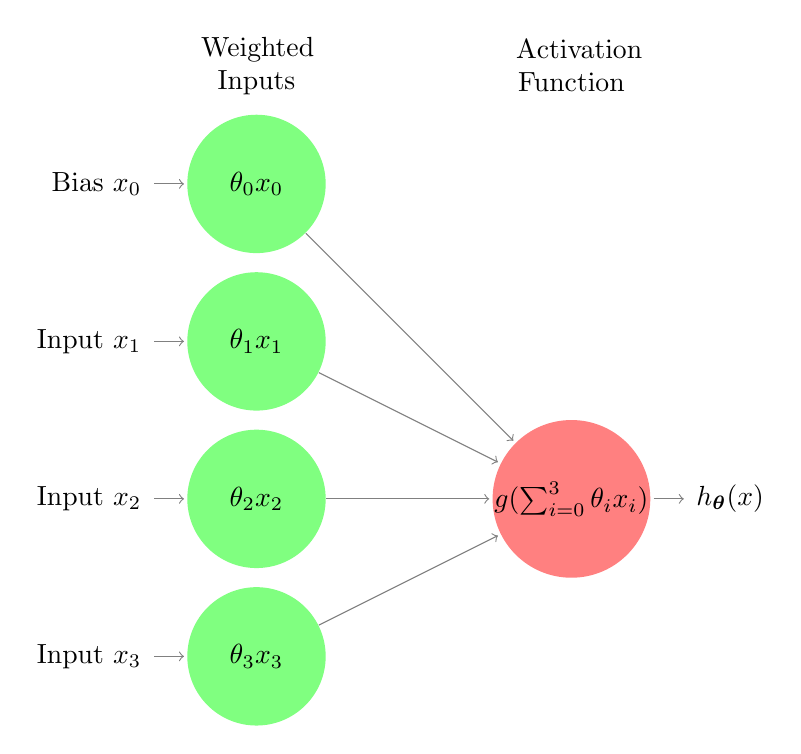
\begin{tikzpicture}[shorten >=1pt,->,draw=black!50, node distance=2.5cm]
    \tikzstyle{every pin edge}=[<-,shorten <=1pt]
    \tikzstyle{neuron}=[circle,fill=black!25,minimum size=50pt,inner sep=0pt]
    \tikzstyle{input neuron}=[neuron, fill=green!50];
    \tikzstyle{output neuron}=[neuron, fill=red!50];
    \tikzstyle{hidden neuron}=[neuron, fill=blue!50];
    \tikzstyle{annot} = [text width=4em, text centered]

    % Draw the input layer nodes
 %   \foreach \name / \y in {0,...,3}
    % This is the same as writing \foreach \name / \y in {1/1,2/2,3/3,4/4}
        \node[input neuron, pin=left:Bias $x_0$] (I-0) at (0,-0) {$\theta_0 x_0$};
	\foreach \name / \y in {1,...,3}
    % This is the same as writing \foreach \name / \y in {1/1,2/2,3/3,4/4}
        \node[input neuron, pin=left:Input $x_{\y}$] (I-\name) at (0,-2*\y) {$\theta_{\y}x_\y$};
    % Draw the hidden layer nodes
    %\foreach \name / \y in {1,...,5}
     %   \path[yshift=0.5cm]
      %      node[hidden neuron] (H-\name) at (\layersep,-\y cm) {};

    % Draw the output layer node
    \node[output neuron,pin={[pin edge={->}]right:$h_{\bm{\theta}}(x)$}, right of=I-2, node distance=4cm] (O) {$g(\sum^3_{i=0}\theta_ix_i)$};

    % Connect every node in the input layer with every node in the
    % hidden layer.
   % \foreach \source in {1,...,4}
    %    \foreach \dest in {1,...,5}
     %       \path (I-\source) edge (H-\dest);

    % Connect every node in the hidden layer with the output layer
    \foreach \source in {0,...,3}
        \path (I-\source) edge (O);

    % Annotate the layers
%    \node[annot,above of=H-1, node distance=1cm] (hl) {Hidden layer};
    \node[annot,above of=I-0, node distance=1.5cm](il) {Weighted Inputs};
    \node[annot,right of=il, node distance=4cm] {Activation Function};
\end{tikzpicture}
\\
The three most common activation functions are:
\begin{itemize}
\item The rectified linear unit or ReLU activation function output is within the range $[0,\infty)$. It has the formula $g(x)=\max\{0,x\}$ corresponding to node function $h_{\bm{\theta}}(\textbf{x})=\max\{0,\bm{\theta}^\top\textbf{x}\}$.
\item The sigmoid or logistic activation function outputs are restricted to $[0,1)$, with the formula $g(x)=(1+\exp(-x))^{-1}$ corresponding to node function  $h_{\bm{\theta}}(\textbf{x})=(1+\exp(-\bm{\theta}^\top\textbf{x}))^{-1}$.
\item The hyperbolic tangent function output ranges between $(-1,1)$, denoted as $g(x)=\tanh(x)$ corresponding to $h_{\bm{\theta}}(\textbf{x})=\tanh(\bm{\theta}^\top\textbf{x})$.
\item The linear activation function is used to describe nodes with no activation function, as its formula is $g(x)=x$, corresponding to $h_{\bm{\theta}}(\textbf{x})=\bm{\theta}^\top\textbf{x}$. It therefore ranges in $(-\infty, \infty)$.
\end{itemize}
A typical neural network is made up of layers of interconnected nodes. The first layer, called the input layer, does not have an activation function or weights, rather it simply acts as an input interface for the network. The outputs from the nodes can only be sent to other nodes in succeeding layers, with the exception of the final output layer; it's result is simply the output of the network. The layers of nodes between the input and output layer are called the hidden layers, as its weights and outputs are not useful to the user. Hidden layers can have any number of nodes, whilst the nodes in the input and output layers are restricted to the number of inputs and outputs the program has. The figure below illustrates a simple neural network with 3 inputs, 1 hidden layer with 3 nodes and 1 output node.\\
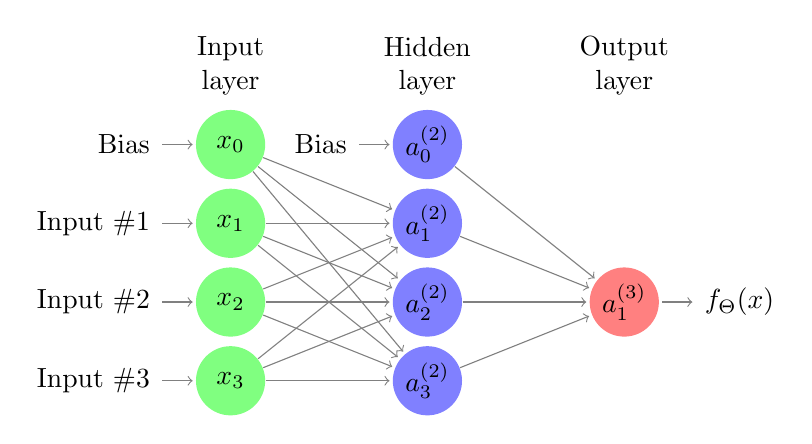
\begin{tikzpicture}[shorten >=1pt,->,draw=black!50, node distance=2.5cm]
    \tikzstyle{every pin edge}=[<-,shorten <=1pt]
    \tikzstyle{neuron}=[circle,fill=black!25,minimum size=25pt,inner sep=0pt]
    \tikzstyle{input neuron}=[neuron, fill=green!50];
    \tikzstyle{output neuron}=[neuron, fill=red!50];
    \tikzstyle{hidden neuron}=[neuron, fill=blue!50];
    \tikzstyle{annot} = [text width=4em, text centered]
    
	\node[input neuron, pin=left:Bias] (I-0) at (0,0) {$x_0$};
    % Draw the input layer nodes
    \foreach \name / \y in {1,...,3}
    % This is the same as writing \foreach \name / \y in {1/1,2/2,3/3,4/4}
        \node[input neuron, pin=left:Input \#\y] (I-\name) at (0,-\y) {$x_\y$};

 \path[yshift=0cm]
            node[hidden neuron, pin=left:Bias] (H-0) at (2.5cm,0) {$a^{(2)}_0$};
    % Draw the hidden layer nodes
    \foreach \name / \y in {1,...,3}
        \path[yshift=0cm]
            node[hidden neuron] (H-\name) at (2.5cm,-\y) {$a^{(2)}_\y$};

    % Draw the output layer node
	\path[yshift=1cm]    
    node[output neuron,pin={[pin edge={->}]right:$f_\Theta(x)$}, right of=H-2] (O) {$a_1^{(3)}$};

    % Connect every node in the input layer with every node in the
    % hidden layer.
    \foreach \source in {0,...,3}
        \foreach \dest in {1,...,3}
            \path (I-\source) edge (H-\dest);

    % Connect every node in the hidden layer with the output layer
    \foreach \source in {0,...,3}
        \path (H-\source) edge (O);

    % Annotate the layers
    \node[annot,above of=H-0, node distance=1cm] (hl) {Hidden layer};
    \node[annot,left of=hl] {Input layer};
    \node[annot,right of=hl] {Output layer};
\end{tikzpicture}\\
In this example, we denote the activation function as $g$, the output of unit $i$ in layer $j$ as $a^{(j)}_i$, and the matrix of weights from layer $j$ to $j+1$ as $\Theta^{(j)}$. We also use the subscript $\Theta^{(j)}_{m,n}$ where $m$ is the row of the matrix corresponding to the unit $m$ in layer $j+1$, and $n$ is the column of the matrix relating to unit $n$ in layer $j$.\\
Individually, the outputs in the hidden nodes and the output node are:
\[x_0=1,\qquad a_0^{(2)}=1\]
\[a_1^{(2)}=g(\Theta^{(1)}_{1,0}x_0+\Theta^{(1)}_{1,1}x_1+\Theta^{(1)}_{1,2}x_2+\Theta^{(1)}_{1,3}x_3)\]
\[a_2^{(2)}=g(\Theta^{(1)}_{2,0}x_0+\Theta^{(1)}_{2,1}x_1+\Theta^{(1)}_{2,2}x_2+\Theta^{(1)}_{2,3}x_3)\]
\[a_3^{(2)}=g(\Theta^{(1)}_{3,0}x_0+\Theta^{(1)}_{3,1}x_1+\Theta^{(1)}_{3,2}x_2+\Theta^{(1)}_{3,3}x_3)\]
\[f_\Theta(\bm{x})=a_1^{(3)}=g(\Theta^{(2)}_{1,0}a_0^{(2)}+\Theta^{(2)}_{1,1}a_1^{(2)}+\Theta^{(2)}_{1,2}a_2^{(2)}+\Theta^{(2)}_{1,3}a_3^{(2)})\]
Denoting the weights outputting to unit $i$ in layer $j+1$ as $\bm{\theta}^{(j)}_i = [\Theta_{i,0}^{(j)}\quad \Theta_{i,1}^{(j)}\dots \Theta_{i,k}^{(j)}]^\top$ where $k+1$ is the number of inputs, we have the vectorized notation:
\[a_0^{(2)}=1\]
\[a_1^{(2)}=g(\bm{\theta}^{(1)^\top}_1\bm{x})\]
\[a_2^{(2)}=g(\bm{\theta}^{(1)^\top}_2\bm{x})\]
\[a_3^{(2)}=g(\bm{\theta}^{(1)^\top}_3\bm{x})\]
\[f_{\bm{\theta}}(\bm{x})=a_1^{(3)}=g(\bm{\theta}_1^{(2)^\top}\bm{a}^{(2)})\] 
where $\bm{a}^{(2)}=[a_0^{(2)}\quad a_1^{(2)}\quad a_2^{(2)}\quad a_3^{(3)}]^\top$.\\
An even simpler notation is:
\[a_0^{(2)}=1\]
\[[a_1^{(2)}\quad a_2^{(2)}\quad a_3^{(2)}]=g(\Theta^{(1)^\top}\bm{x})\]
\[f_\Theta (\bm{x})=\bm{a}^{(3)}=g(\Theta^{(2)^\top}\bm{a}^{(2)})\]
\subsubsection{Bias-per-node Representation}
In practice, the bias node is often replaced with an intercept term added to the weighted input of a node before it passes through the activation function. These intercept terms are optimized alongside the weights. This representation is preferred in code as it makes the dimensionality of the weight matrices consistent, as the number of inputs of a layer becomes equal to the number of outputs of the previous layer. In both cases, the bias takes the form of a flat value added to the weighted inputs, which can be optimized, so there is no practical difference between these two notations. The sum of intercept terms in a layer is equivalent to the weight corresponding to a bias node for the layer. Below, we repeat the example of an individual node with three inputs, but with an individual intercept $b_i$ per node.\\
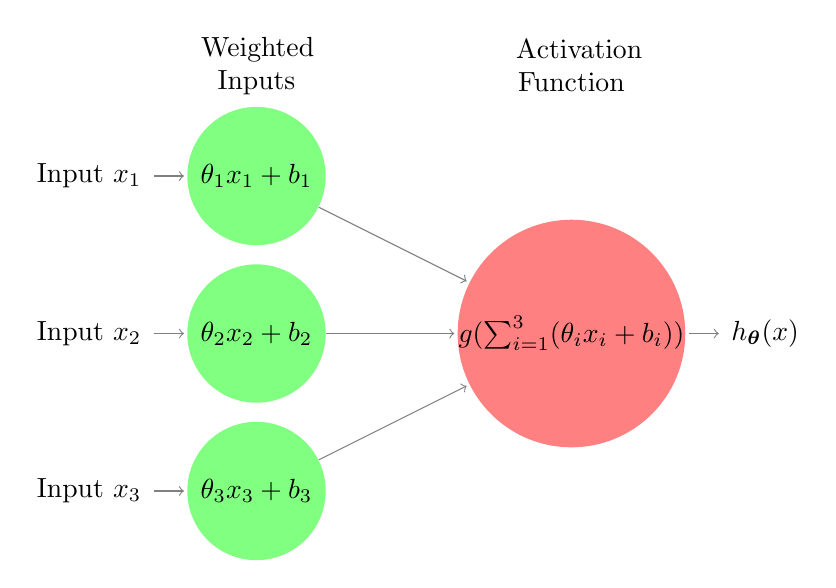
\begin{tikzpicture}[shorten >=1pt,->,draw=black!50, node distance=2.5cm]
    \tikzstyle{every pin edge}=[<-,shorten <=1pt]
    \tikzstyle{neuron}=[circle,fill=black!25,minimum size=50pt,inner sep=0pt]
    \tikzstyle{input neuron}=[neuron, fill=green!50];
    \tikzstyle{output neuron}=[neuron, fill=red!50];
    \tikzstyle{hidden neuron}=[neuron, fill=blue!50];
    \tikzstyle{annot} = [text width=4em, text centered]

    % Draw the input layer nodes
 %   \foreach \name / \y in {0,...,3}
    % This is the same as writing \foreach \name / \y in {1/1,2/2,3/3,4/4}
      %  \node[input neuron, pin=left:Bias $x_0$] (I-0) at (0,-0) {$\theta_0 x_0$};
	\foreach \name / \y in {1,...,3}
    % This is the same as writing \foreach \name / \y in {1/1,2/2,3/3,4/4}
        \node[input neuron, pin=left:Input $x_{\y}$] (I-\name) at (0,-2*\y) {$\theta_{\y}x_\y+b_\y$};
    % Draw the hidden layer nodes
    %\foreach \name / \y in {1,...,5}
     %   \path[yshift=0.5cm]
      %      node[hidden neuron] (H-\name) at (\layersep,-\y cm) {};

    % Draw the output layer node
    \node[output neuron,pin={[pin edge={->}]right:$h_{\bm{\theta}}(x)$}, right of=I-2, node distance=4cm] (O) {$g(\sum^3_{i=1}(\theta_ix_i+b_i))$};

    % Connect every node in the input layer with every node in the
    % hidden layer.
   % \foreach \source in {1,...,4}
    %    \foreach \dest in {1,...,5}
     %       \path (I-\source) edge (H-\dest);

    % Connect every node in the hidden layer with the output layer
    \foreach \source in {1,...,3}
        \path (I-\source) edge (O);

    % Annotate the layers
%    \node[annot,above of=H-1, node distance=1cm] (hl) {Hidden layer};
    \node[annot,above of=I-1, node distance=1.4cm](il) {Weighted Inputs};
    \node[annot,right of=il, node distance=4cm] {Activation Function};
\end{tikzpicture} \\
Note here that $\sum^3_{i=1}b_i=\theta_0x_0$. The representation of the simple neural network example in the previous section becomes:
\[a_1^{(2)}=g(\Theta^{(1)}_{1,1}x_1+b^{(1)}_1+\Theta^{(1)}_{1,2}x_2+b^{(1)}_2+\Theta^{(1)}_{1,3}x_3+b^{(1)}_3)\]
\[a_2^{(2)}=g(\Theta^{(1)}_{2,1}x_1+b^{(1)}_1+\Theta^{(1)}_{2,2}x_2+b^{(1)}_2+\Theta^{(1)}_{2,3}x_3+b^{(1)}_3)\]
\[a_3^{(2)}=g(\Theta^{(1)}_{3,1}x_1+b^{(1)}_1+\Theta^{(1)}_{3,2}x_2+b^{(1)}_2+\Theta^{(1)}_{3,3}x_3+b^{(1)}_3)\]
\[f_\Theta(\bm{x})=a_1^{(3)}=g(\Theta^{(2)}_{1,1}a_1^{(2)}+b^{(2)}_1+\Theta^{(2)}_{1,2}a_2^{(2)}+b^{(2)}_2+\Theta^{(2)}_{1,3}a_3^{(2)}+b^{(2)}_3)\]
or in vectorized notation,
\[\bm{a}^{(2)}=g(\Theta^{(1)^\top}\bm{x})\]
\[f_\Theta(\bm{x})=\bm{a}^{(3)}=g(\Theta^{(2)^\top}\bm{a}^{(2)})\]
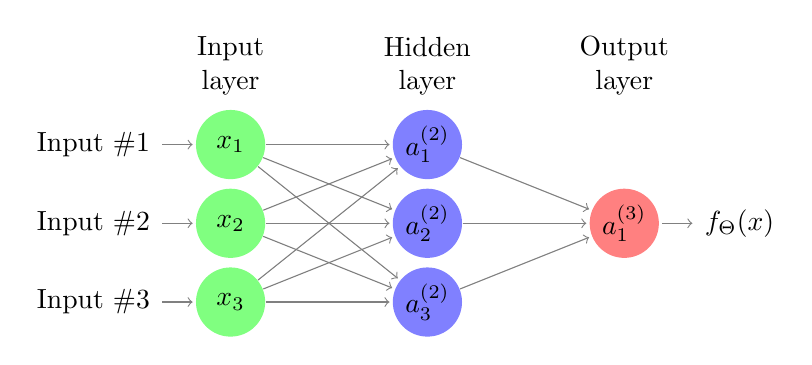
\begin{tikzpicture}[shorten >=1pt,->,draw=black!50, node distance=2.5cm]
    \tikzstyle{every pin edge}=[<-,shorten <=1pt]
    \tikzstyle{neuron}=[circle,fill=black!25,minimum size=25pt,inner sep=0pt]
    \tikzstyle{input neuron}=[neuron, fill=green!50];
    \tikzstyle{output neuron}=[neuron, fill=red!50];
    \tikzstyle{hidden neuron}=[neuron, fill=blue!50];
    \tikzstyle{annot} = [text width=4em, text centered]
    
	%\node[input neuron, pin=left:Bias] (I-0) at (0,0) {$x_0$};
    % Draw the input layer nodes
    \foreach \name / \y in {1,...,3}
    % This is the same as writing \foreach \name / \y in {1/1,2/2,3/3,4/4}
        \node[input neuron, pin=left:Input \#\y] (I-\name) at (0,-\y) {$x_\y$};

 %\path[yshift=0cm]
  %          node[hidden neuron, pin=left:Bias] (H-0) at (2.5cm,0) {$a^{(2)}_0$};
    % Draw the hidden layer nodes
    \foreach \name / \y in {1,...,3}
        \path[yshift=0cm]
            node[hidden neuron] (H-\name) at (2.5cm,-\y) {$a^{(2)}_\y$};

    % Draw the output layer node
	\path[yshift=1cm]    
    node[output neuron,pin={[pin edge={->}]right:$f_\Theta(x)$}, right of=H-2] (O) {$a_1^{(3)}$};

    % Connect every node in the input layer with every node in the
    % hidden layer.
    \foreach \source in {1,...,3}
        \foreach \dest in {1,...,3}
            \path (I-\source) edge (H-\dest);

    % Connect every node in the hidden layer with the output layer
    \foreach \source in {1,...,3}
        \path (H-\source) edge (O);

    % Annotate the layers
    \node[annot,above of=H-1, node distance=1cm] (hl) {Hidden layer};
    \node[annot,left of=hl] {Input layer};
    \node[annot,right of=hl] {Output layer};
\end{tikzpicture}
\newpage
\subsubsection{Choice of Activation Function}
Recall in section idk the three most common activation functions:
\begin{itemize}
\item The rectified linear unit or ReLU activation function $g(x)=\max\{0,x\}$ ranging in $[0,\infty)$.
\item The sigmoid or logistic activation function $g(x)=(1+\exp(-x))^{-1}$ restricted to $[0,1)$.
\item The hyperbolic tangent function $g(x)=\tanh(x)$ ranging between $(-1,1)$.
\item The linear activation function $g(x)=x$ ranging in $(-\infty, \infty)$.
\end{itemize}
In deep learning, rectified linear units are the default choice for the hidden layers for their many advantages:
\begin{itemize}
\item Reduces overfitting: since negative ReLU inputs result in a zero output, only half of the units are "active" (non-zero output) when the network is first initialized. The proportion of active units can increase or decrease during training such that overfitting and underfitting is minimized.
\item Faster computation: a $\max\{0,x\}$ function is computed much faster than a function that uses $\exp$ or $\tanh$.
\item Easier and more consistent training: weight training in a neural network (discussed in the next section) uses the gradient of overall node function, which is influenced by the activation function. The rectified linear unit has a consistent gradient $(1\times \theta)$ or $(0\times \theta)$ resulting in consistent training, as opposed to more complex units. 
\end{itemize}
As described in section , the input layer has no activation function, so it can be described as having a linear activation function.\\
For the output layer, the activation function with the most reasonable output range is used. This depends on what the network is being used for. For example, in classification, the network assigns a probability to each case, so a sigmoid activation function would be most reasonable, as it ranges between 0 and 1. On the other hand, a rectified linear unit would be used for regression of a non-negative quantity such as price or time.
\newpage
\subsubsection{Optimization}
The goal of optimizing the network is to train the weights of the network such that a loss function, which we will denote as $L$ as minimized. A common loss function is the squared error between the batch of network outputs and the actual results:
\[\min_\Theta L(\Theta)=\frac12 (\bm{y}-\bm{f}_\Theta(\bm{x}))^\top(\bm{y}-\bm{f}_\Theta(\bm{x})).\]
The $\frac12$ factor is included to eliminate the factor of 2 in the derivative, simplifying the derivations. The derivative is multiplied by an arbitrary training rate during optimization so there is no significant impact of including that term.\\
The weights are initialized randomly, and their values are used to calculate the partial derivative of the loss function with respect to each individual weight (and intercept). These partial derivatives are used in the gradient-based optimization of the weights. There are many variations of neural network optimization algorithms, but they are all based off gradient descent, which we will cover in this section.\\
Gradient descent is an algorithm used to find the minimizer $\bm{x}^*$ of a function $f$ by iterating on an arbitrary point $\bm{x}^{(n)}$, taking steps proportional to a descent direction $\bm{s}^{(n)}$:
\[\bm{x}^{(n+1)}=\bm{x}^{(n)}+\alpha \bm{s}^{(n)},\qquad \alpha>0.\] 
\textbf{Definition:} At point $\bm{x}^{(n)}$, $\bm{s}^{(n)}$ is a descent direction if $\nabla f(\bm{x}^{(n)})^\top \bm{s}^{(n)}<0$.\\
\textbf{Preposition:} If $\bm{s}^{(n)}$ is a descent direction, then for small $\alpha>0$, $f(\bm{x}^{(n)}+\alpha \bm{s}^{(n)})<f(\bm{x}^{(n)})$.\\
Proof: (proof copied from jeyakumar optimization lecture notes topic 6)\\
First we show that
\[\frac{d}{d\alpha}f(\bm{x}^{(n)}+\alpha \bm{s}^{(n)})=\nabla f(\bm{x}^{(n)}+\alpha \bm{s}^{(n)})^\top \bm{s}^{(n)}.\]
where $\bm{x}^{(n)}=[x_1^{(n)},\dots,x_n^{(k)}]^\top$ and $\bm{s}^{(k)}=[s_1^{(n)},\dots,s_k^{(n)}]^\top$.\\
Let
\[x_i^{(n)}(\alpha)=x_i^{(n)}+\alpha s_i^{(n)},\quad i=1,\dots,n\]
so that $\bm{x}^{(n)}+\alpha \bm{s}^{(n)}=[x_1^{(n)}(\alpha),\dots,x_k^{(n)}(\alpha)]^\top$.
We have
\begin{align*}
\frac{d}{d\alpha}f(\bm{x}^{(n)}+\alpha\bm{s}^{(n)})&= \frac{d}{d\alpha}f(x_1^{(n)},\dots,x_k^{(n)}(\alpha))\\
&= \frac{\partial f(\bm{x})}{\partial x_1}|_{\bm{x}=\bm{x}^{(n)}+\alpha \bm{s}^{(n)}}\frac{d(x_1^{(n)}(\alpha)}{d\alpha}+\dots+\frac{\partial f(\bm{x})}{\partial x_k}|_{\bm{x}=\bm{x}^{(n)}+\alpha \bm{s}^{(n)}}\frac{d(x_k^{(n)}(\alpha)}{d\alpha}\\
&=\frac{\partial f(\bm{x})}{\partial x_1}|_{\bm{x}=\bm{x}^{(n)}+\alpha \bm{s}^{(n)}}\bm{s}_1^{(n)}+\dots+\frac{\partial f(\bm{x})}{\partial x_n}|_{\bm{x}=\bm{x}^{(n)}+\alpha \bm{s}^{(n)}}\bm{s}_k^{(n)}\\
&=\nabla f(\bm{x}^{(n)}+\alpha \bm{s}^{(n)})^\top \bm{s}^{(n)}
\end{align*}
Setting $\alpha=0$ and using definition (),
\[\frac{d}{d\alpha}f(\bm{x}^{(n)}+\alpha\bm{s}^{(n)})|_{\alpha=0}=\nabla f(\bm{x}^{(n)})^\top \bm{s}^{(n)}<0\]
Therefore for small $\alpha>0$,
\[f(x^{(n)}+\alpha s^{(n)})<f(x^{(n)}).\]
QED.\\
\\
A common choice of descent direction is the negative of the gradient $-\nabla f(\bm{x}^{(n)})$, leading to the method of steepest descent. It is clearly a descent direction as $-\nabla f(\bm{x}^{(n)})^\top\nabla f(\bm{x}^{(n)})=-||\nabla f(\bm{x}^{(n)})||^2<0$.\\
By nature, gradient descent is guaranteed to converge to a local minimum, which is problematic if the function has local minima which differ from the global minima. This is not an issue in this thesis, as all the loss functions we use are convex, so any local minima are also global minima. Those interested in global optimization can refer to (Deterministic Global Optimization, Floudas). When training a neural network on a non-convex loss function there are currently no commonly used methods of guaranteeing a global minimum, but the path may escape from a local minimum if randomness is introduced to the training process. This can be accomplished by stochastic gradient descent.\\
Typically, the entire batch of data is used in each iteration to calculate the loss function and gradient values required for gradient descent. This method of batch gradient descent is very slow for large datasets, and as previously described, its smoothness can cause the algorithm to converge to local minima. In stochastic gradient descent, only one observation is used per iteration, so the latent randomness associated with each observation effectively leads to noise added to each step. In practice, a compromise between stochastic and batch gradient descent is typically used; mini-batch gradient descent involves using several observations per iteration, leading to a reduction in the gradient variance.\\
Gradient descent convergence can be improved by using an adaptive learning rate (ie. decreasing $\alpha$ over the iterations), as a low learning rate in the process will make convergence slow, whilst a high learning rate can cause the algorithm to oscillate around the minima.\\
The Adam algorithm (Kingma, Ba 2014) incorporates these two concepts to form an effective optimization algorithm that is widely used to optimize neural networks. In this thesis, we use this algorithm, but omit the specifics as they are beyond the scope of this thesis.
\newpage
\subsubsection{Back-propogation}
In the back-propogation algorithm, the goal is to find the partial derivative of the loss function with respect to the individual weights \[\frac{\partial}{\partial\Theta_{m,n}^{(j)}}L(\Theta),\]
so that gradient descent can be performed to optimize the weights. For each training sample $(\bm{x}^{(I)},\bm{y}^{(I)})$, $I=1,\dots,N$, the input signal is propogated forward throughout the network to calculate $\bm{a}^{(j)}$ for $j=2,\dots,J$, where $J$ is the total number of layers. The difference between the network output and the ideal result is calculated with 
\[\bm{\delta}^{(J)}=\bm{a}^{(J)}-\bm{y}^{(I)},\] 
and this error is propogated backwards through the network to find $\bm{\delta}^{(J-1)},\dots,\bm{\delta}^{(2)}$ by using the formula 
\[\bm{\delta}^{(j)}=((\Theta^{(j)})^\top \bm{\delta}^{(j+1)}).*g'(\Theta^{(j)^\top} \bm{a}^{(j)}),\] 
where $.*$ denotes element-wise multiplication and $g'$ is the derivative of the activation function. In this case, $g'$ takes in the sum of its weighted inputs, and as an example, the sigmoid activation function has the derivative $g'(\Theta^{(j)^\top} \bm{a}^{(j)})=\bm{a}^{(j)}.*(1-\bm{a}^{(j)})$. Note that $\bm{\delta}^{(1)}$ does not need to be calculated as the input layer is not weighted. \\
The errors for each layer are multiplied by each of the preceeding layer's activation outputs to form the estimated partial derivative for the training sample. This result is added to an accumulator matrix, so that the average partial derivative from all the training samples can be computed:
\[\Delta^{(j)}_{m,n}:=\Delta^{(j)}_{m,n}+a_n^{(j)}\delta_m^{(j+1)}\]
or in matrix-vector form.
\[\Delta^{(j)}:=\Delta^{(j)}+\bm{\delta}^{(j+1)}(\bm{a}^{(j)})^\top.\]
Finally, we divide the accumulator matrix entries by the number of training samples to find the average partial derivative of the cost function with respect to the weights:
\[\frac{\partial}{\partial \Theta^{(j)}_{m,n}}L(\Theta)=\frac1N \Delta_{m,n}^{(j)}\]
When $n\neq0$ (i.e. not considering the bias node), we can optionally add a regularizer term $\lambda > 0$ which decreases the magnitude of the weights, preventing overfitting. 
\[\frac{\partial}{\partial \Theta^{(j)}_{m,n}}L(\Theta)=\frac1N (\Delta_{m,n}^{(j)}+\lambda \Theta_{m,n}^{(j)})\]
There is no significant change when the bias node is regularized.\\
Pseudocode for the back-propogation algorithm is shown below.\\
\begin{algorithm}
\caption{Back-Propogation Algorithm}
\KwData{Training Data $\{(\bm{x}^{(1)},\bm{y}^{(1)}),\dots ,(\bm{x}^{(N)},\bm{y}^{(N)})\}$, Regularizer Term $\lambda$}
\KwResult{Cost Function Partial Derivatives $\frac{\partial}{\partial\Theta^{(j)}_{m,n}}L(\Theta)$}
\BlankLine
\Begin{Randomly initialize weights $\Theta$\;
Set $\Delta^{(j)}_{m,n}=0 \quad \forall j,m,n$\;
\For{$I=1$ \KwTo $N$}{
Set $\bm{a}^{(1)}=\bm{x}^{(I)}$\;
\For{$j=2$ \KwTo $J$}{
Set $\bm{a}^{(j)}=\Theta^{(j-1)^\top}\bm{a}^{(j-1)}$\;}
Set $\bm{\delta}^{(J)}=\bm{a}^{(J)}-\bm{y}^{(I)}$\;
\For{$j=J-1$ \KwTo $2$}{
Set $\bm{\delta}^{(j)}=((\Theta^{(j)})^\top \bm{\delta}^{(j+1)}).*g'(\Theta^{(j)^\top}\bm{a}^{(j)})$\;
}
\For{$j=1$ \KwTo $J-1$}{
Set $\Delta^{(j)}=\Delta^{(j)}+\bm{\delta}^{(j+1)}(\bm{a}^{(j)})^\top$\;
}}
\For{all $j,m,n$}{
\eIf{$n=0$}{Set $\frac{\partial}{\partial\Theta^{(j)}_{m,n}}L(\Theta)=\frac1N \Delta^{(j)}_{m,n}$\;
}{Set $\frac{\partial}{\partial\Theta^{(j)}_{m,n}}L(\Theta)=\frac1N (\Delta^{(j)}_{m,n}+\lambda\Theta^{(j)}_{m,n})$\;}}}
\end{algorithm}
Having derived the partial derivatives of the loss function with respect to the individual weights, we can use gradient descent or some other optimization method to update the weights. The partial derivatives are re-calculated after each optimization update until convergence.
\newpage
\subsubsection{Weight Initialization}
Proper initialization of the weights is ideal to improve convergence, as if the weights are too low, then the nodal outputs will continually decrease through the layers and become very small, requiring many iterations of back-propogation training to fix. Similarly, if the weights are too high, then the result output of forward propogation will be extremely large. In this section we discuss Xavier Initialization, which aims to keep the signal variance constant throughout the network. To derive the initialization algorithm, first consider a single node with $n$ inputs, and let $z$ denote the weighted sum of the inputs $\bm{\theta}^\top\textbf{x}$ before it is passed through the activation function. This is written as
\[z=\theta_0x_0+\theta_1x_1+\dots+\theta_nx_n.\]
$x_0$ is a constant term, so $\Var(\theta_0x_0)=0$. Now under the assumption that the inputs and weights have 0 mean, we find the variance of the other terms:
\[\Var(\theta_ix_i)=\E[x_i]^2\Var(\theta_i)+\E[\theta_i]^2\Var(x_i)+\Var(\theta_i)\Var(x_i)=\Var(\theta_i)\Var(x_i).\]
Assuming that the weights and inputs are also independent and identically distributed, we have
\[\Var(z)=n\Var(\theta_i)\Var(x_i).\]
Since we want constant variance of the signals throughout the network, we set $\Var(z)=\Var(x_i)$ and the result follows:
\[\Var(\theta_i)=\frac1n.\]
However, this result only considers forward propogation of the signal. A variation of this result accounts for back propogation by averaging the number of input and output nodes:
\[\Var(\theta_i)=\frac{2}{n_{in}+n_{out}}.\]
Thus, to enforce constant signal variance throughout the network, the ideal initialization of weights is to sample from a distribution, typically uniform or Gaussian, with $0$ mean and $\frac{2}{n_{in}+n_{out}}$ variance:
\[\theta_i\sim U\left(-\sqrt{\frac{6}{n_{in}+n_{out}}},\sqrt{\frac{6}{n_{in}+n_{out}}}\right)\]
or
\[\theta_i\sim N\left(0,\frac{2}{n_{in}+n_{out}}\right).\]
\subsubsection{References}
http://proceedings.mlr.press/v9/glorot10a/glorot10a.pdf\\
Machine Learning by Andrew Ng Stanford online course\\
\newpage
\subsection{Kernel Density Estimation}
Kernel density estimation is a non-parametric method used to estimate the probability density function of a distribution, using only samples. It can therefore be used to estimate implicit distributions. For simplicity we only explain the univariate form of the kernel density estimator, though the multivariate form is used in this thesis.\\
\\
Let $\{x^{(i)}\}^n_{i=1}$ be an independent and identically distributed sample from a distribution with unknown probability density function $f$. Its kernel density estimator is defined as
\[\hat{f}_h(x)=\frac{1}{nh}\sum^n_{i=1}K\left(\frac{x-x^{(i)}}{h}\right).\]
$K$ is the kernel, a symmetric non-negative weighting function that integrates to 1. Examples of kernel functions are:
\begin{itemize}
\item Epanechnikov: $K(u)=\frac{3}{4}(1-u^2), |u|\leq 1$
\item Uniform: $K(u)=\frac12, |u|\leq 1$
\item Gaussian: $K(u)=\frac{1}{\sqrt{2\pi}}\exp\left(-\frac{1}{2}u^2\right)$.
\end{itemize}
Typically, the Gaussian kernel is used due to its statistical properties, but the choice of kernel is not as important as the choice of $h$, the bandwidth.\\
\\
The bandwidth $h>0$ acts as a smoothing parameter, determining the width of the kernel. If $h$ is too small, $\hat{f}$ will be 'undersmoothed' as too much weight is placed on the areas nearest the data-points, leading to a spiky estimate with high variance. On the other hand, if $h$ is too large, $\hat{f}$ will be 'oversmoothed' with too little weight on areas nearest to the data-points, resulting in a relatively flat estimate with high bias. It is therefore ideal to choose $h$ such that the mean integrated square error $MISE(h)=\E\left[\int(\hat{f}_h(x)-f(x))^2dx\right]$ is minimized. For a Gaussian kernel, this is approximately $h=1.06\hat{\sigma}n^{-1/5}$ where $\hat{\sigma}$ is the sample standard deviation. We omit the proof in this thesis.\\
\\
The kernel density estimator works by placing a kernel on each data point and summing up the kernels to produce a smooth curve. Each point on the curve is essentially a weighted average of nearby data points. Regions of the curve with many data points will therefore have a high estimated probability density.
\newpage
\subsection{Variational Inference}
\subsubsection{Context}
In Bayesian statistics, a common problem is to estimate posterior densities, so that we may perform inference to determine an unknown parameter. Consider a set of unknown, latent variables $\textbf{Z}=\{z_i\}^M_{i=1}$ and a dataset of known variables $\textbf{X}=\{x_i\}^N_{i=1}$. These sets have a joint density of $P(\textbf{Z},\textbf{X})$. In the Bayesian framework, inference is often performed on the posterior density (the distribution of the parameters $\textbf{Z}$ after the data $\textbf{X}$ is observed)
$P(\textbf{Z}|\textbf{X})$, which, after applying Bayes' theorem, can be written as:
\begin{equation*}P(\textbf{Z}|\textbf{X})=\frac{P(\textbf{Z})P(\textbf{X}|\textbf{Z})}{P(\textbf{X})}= \frac{P(\textbf{Z})P(\textbf{X}|\textbf{Z})}{\int_\mathcal{Z}P(\textbf{Z},\textbf{X})d\textbf{Z}}\end{equation*}
where
\begin{itemize}
\item $P(\textbf{Z})$ is the prior distribution: the initial distribution of $\textbf{Z}$ before the data $\textbf{X}$ is observed. This can be initialised to represent our initial beliefs, or it can be parametrised randomly,
\item $P(\textbf{X}|\textbf{Z})$ is the likelihood: the distribution of data $\textbf{X}$ conditioned on the parameters $\textbf{Z}$,
\item $P(\textbf{X})=\int_\mathcal{Z}P(\textbf{Z},\textbf{X})d\textbf{Z}$ is the marginal likelihood, or the evidence: the density of the data averaged across all possible parameter values.
\end{itemize}
If the evidence integral $P(\textbf{X})=\int_\mathcal{Z}P(\textbf{Z},\textbf{X})d\textbf{Z}$ is impossible or difficult to compute (possibly because it is unavailable in closed form or the dimensionality is too high), then we are unable to evaluate the posterior density. Traditionally, MCMC(Markov Chain Monte Carlo) methods overcome this obstacle by constructing a Markov chain that converges to the stationary distribution $P(\textbf{Z}|\textbf{X})$, then sampling from the chain to create an empirical estimate for the posterior distribution. However, these methods rely on the speed of convergence, which can be slow for large datasets or complex models. When faced with these issues or when desiring a faster computation, one may instead apply variational inference, an alternative approach to density estimation.
\subsubsection{Introduction to Variational Inference}
Variational inference chooses another distribution $Q(\textbf{Z})$ from a select family of variational distributions (approximate densities) $\mathcal{Q}$ to serve as an approximation to $P(\textbf{Z}|\textbf{X})$, and then minimizes the divergence between the two distributions in an optimization problem:
\begin{equation}
Q^*(\textbf{Z})=\argmin_{Q(\textbf{Z})\in \mathcal{Q}}D(Q(\textbf{Z})||P(\textbf{Z}|\textbf{X}))
\end{equation} where $D$ denotes an f-divergence (a measure of how divergent two probability distributions are, it is minimized if $Q=P$). This results in an analytical approximation to the posterior density. Additionally, a lower bound for the marginal likelihood of the dataset is derived, which can be used as a model selection criterion. Due to the stochastic nature of the optimization, variational inference methods can be much faster than MCMC, but the solution is only locally optimal as there is no guarantee of global convergence.
\subsubsection{Derivation of the ELBO}
The most common f-divergence used in variational inference is the KL(Kullback-Leibler) divergence, defined as the expected logarithmic difference between two distrbutions $Q$ and $P$ with respect to $Q$:
\begin{equation*}
KL(Q||P)=\int_{-\infty}^\infty Q(x)\log \frac{Q(x)}{P(x)}dx=\mathbb{E}_{Q(x)}\left[\log\frac{Q(x)}{P(x)}\right].
\end{equation*}
Note that the KL divergence is not symmetric. We use the reverse KL divergence instead of the forward KL divergence $KL(P||Q)$ because it leads to an expectation maximization algorithm as opposed to an expectation propagation algorithm.\\
Using this expression, we can rewrite equation (1) as:
\begin{align*}
Q^*(\textbf{Z})&=\argmin_{Q(\textbf{Z})\in \mathcal{Q}}KL(Q(\textbf{Z})||P(\textbf{Z}|\textbf{X}))\\
&= \argmin_{Q(\textbf{Z})\in \mathcal{Q}} \mathbb{E}_{Q(\textbf{Z})}[\log Q(\textbf{Z})-\log P(\textbf{Z}|\textbf{X})]\\
&= \argmin_{Q(\textbf{Z})\in \mathcal{Q}} \mathbb{E}_{Q(\textbf{Z})}\left[\log Q(\textbf{Z})-\log\frac{P(\textbf{X}|\textbf{Z})P(\textbf{Z})}{P(\textbf{X})}\right]\\
&= \argmin_{Q(\textbf{Z})\in \mathcal{Q}} \left(\mathbb{E}_{Q(\textbf{Z})}[\log Q(\textbf{Z})-\log P(\textbf{X}|\textbf{Z})-\log P(\textbf{Z})]+\log P(\textbf{X})\right).
\end{align*}
Note in the last line $\mathbb{E}_{Q(\textbf{Z})}[P(\textbf{X})]=P(\textbf{X})$ as it is not dependent on $Q(\textbf{Z})$. Also note that the KL divergence is dependent on $P(\textbf{X})$, which we have determined to be intractable, so this optimization problem cannot be solved in this form. This issue is resolved by rearranging the KL divergence expression as follows:
\begin{align}
KL(Q(\textbf{Z})||P(\textbf{Z}|\textbf{X}))&=\mathbb{E}_{Q(\textbf{Z})}[\log Q(\textbf{Z})-\log P(\textbf{X}|\textbf{Z})-\log P(\textbf{Z})]+\log P(\textbf{X}) \nonumber \\
\log P(\textbf{X})-KL(Q(\textbf{Z})||P(\textbf{Z}|\textbf{X}))&=-\mathbb{E}_{Q(\textbf{Z})}[\log Q(\textbf{Z})-\log P(\textbf{X}|\textbf{Z})-\log P(\textbf{Z})]\nonumber \\
&=\mathbb{E}_{Q(\textbf{Z})}[\log P(\textbf{X}|\textbf{Z})]-\mathbb{E}_{Q(\textbf{Z})}[\log Q(\textbf{Z})-\log P(\textbf{Z})]\nonumber \\
&=\mathbb{E}_{Q(\textbf{Z})}[\log P(\textbf{X}|\textbf{Z})]-KL(Q(\textbf{Z})||P(\textbf{Z})).
\end{align}
We refer to $\log P(\textbf{X})-KL(Q(\textbf{Z})||P(\textbf{Z}|\textbf{X}))$ as $ELBO(Q)$ (evidence lower bound), as it is equal to the marginal probability of the data subtracted by a constant error term. This error term $KL(Q(\textbf{Z})||P(\textbf{Z}|\textbf{X}))$ becomes 0 when $Q(\textbf{Z})=P(\textbf{Z}|\textbf{X})$, maximizing the ELBO. Note that since $P(\textbf{X})$ is constant, maximizing the $ELBO$ is equal to minimizing the KL divergence between $Q(\textbf{Z})$ and $P(\textbf{Z}|\textbf{X})$, and that the expression on line (2) is entirely computable. We can therefore rewrite our optimization problem from equation (1) as:
\begin{align*}
Q^*(\textbf{Z})&=\argmin_{Q(\textbf{Z})\in \mathcal{Q}}D(Q(\textbf{Z})||P(\textbf{Z}|\textbf{X}))\\
&= \argmax_{Q(\textbf{Z})\in \mathcal{Q}} ELBO(Q)\\
&= \argmax_{Q(\textbf{Z})\in \mathcal{Q}} \left(\mathbb{E}_{Q(\textbf{Z})}[\log P(\textbf{X}|\textbf{Z})]-KL(Q(\textbf{Z})||P(\textbf{Z}))\right).
\end{align*}
\subsubsection{Mean-Field Variational Family (need to fix notations)}
The family of variational distributions $\mathcal{Q}$ is typically a 'mean-field variational family', in which the distribution $Q(\textbf{Z})$ factorizes over the latent variables $\{z_i\}^M_{i=1}$, each with an individual set of parameters $\{\phi_i\}^M_{i=1}$:
\begin{equation}
Q(\textbf{Z})=\prod^M_{i=1}q^{(i)}_{\phi_i}(z_i).
\end{equation}
The individual factors $q^{(i)}_{\phi_i}(z_i)$ can take any form, but they are assumed to be independent, which simplifies derivations but is less accurate when the true latent variables exhibit dependence. Fixing the forms of the individual factors, we want to choose the parameters $\phi_i$ so that $ELBO(Q)$ is maximized. Since the density of the true posterior is dependent on the value of the data point, each data point $x_i$ has its own associated set of parameters. To derive an expression for the optimal factor $q_i^*(z_i)$, we substitute equation (3) into the $ELBO$, factor out a specific $q_j(z_j)$ and equate the functional derivative of the resulting Lagrangian equation with 0. Firstly, we express $ELBO(Q)$ in an integral form as follows:
\begin{align*}
ELBO(Q)&= \mathbb{E}_{Q(Z)}[\log P(\textbf{X}|\textbf{Z})]-KL(Q(\textbf{Z})||P(\textbf{Z}))\\
&= \mathbb{E}_{Q(Z)}[\log P(\textbf{X}|\textbf{Z})+\log P(\textbf{Z})-\log Q(\textbf{Z})]\\
&= \mathbb{E}_{Q(Z)}[\log P(\textbf{X}, \textbf{Z})-\log Q(\textbf{Z})]\\
&= \int_{\mathcal{Z}}Q(\textbf{Z})(\log P(\textbf{X},\textbf{Z})-\log Q(\textbf{Z}))d\textbf{Z}.
\end{align*}
Substituting $Q(\textbf{Z})=\prod^M_{i=1}q_i(z_i)$ and factoring out $q_j(z_j)$ yields:
\begin{align}
ELBO(Q)&= \int_\mathcal{Z}\left[\prod^M_{i=1}q_i(z_i)\right]\left(\log P(\textbf{X},\textbf{Z})-\sum_{i=1}^M\log q_i(z_i)\right)d\textbf{Z}\nonumber\\
&= \int_\mathcal{z_j}q_j(z_j)\left(\int_\mathcal{z_{-j}}\log P(\textbf{X},\textbf{Z})\prod_{i\neq j}q_i(z_i)d\textbf{z}_{-j} \right) dz_j\nonumber\\
&\quad -\int_{\mathcal{z_j}}q_j(z_j)\left(\int_{\mathcal{z}_{-j}}\left[\prod_{i\neq j}q_i(z_i)\right]\sum_{i=1}^M q_i(z_i)d\textbf{z}_{-j}\right)dz_j\nonumber\\
&= \int_{\mathcal{z_j}}q_j(z_j)\mathbb{E}_{\textbf{z}_{-j}}[\log P(\textbf{X},\textbf{Z})]dz_j-\int_{\mathcal{z_j}}q_j(z_j)\log q_j(z_j)\left(\int_{\mathcal{z}_{-j}}\prod_{i\neq j}q_i(z_i)dz_{-j}\right) dz_j\nonumber\\
&\quad -\int_{\mathcal{z_j}}q_j(z_j)\left(\int_{\mathcal{z}_{-j}}\left[\prod_{i\neq j}q_i(z_i)\right]\sum_{i\neq j}q_i(z_i)d{\textbf{z}_{-j}}\right)dz_j\nonumber\\
&= \int_\mathcal{z_j}q_j(z_j)\mathbb{E}_{\textbf{z}_{-j}}[\log P(\textbf{X},\textbf{Z})]dz_j-\int_\mathcal{z_j}q_j(z_j)\log q_j(z_j)dz_j\nonumber\\
&\quad -\int_{\mathcal{z}_{-j}}\left[\prod_{i\neq j}q_i(z_i)\right]\sum_{i\neq j}q_i(z_i)d{\textbf{z}_{-j}}
\\&= \int_\mathcal{z_j}q_j(z_j)\left(\mathbb{E}_{\mathcal{z}_{-j}}[\log P(\textbf{X},\textbf{Z})]-\log q_j(z_j)\right)dz_j+\text{const}.
\end{align}
The term in line (4) becomes a constant as it does not depend on $q_j(z_j)$. Now our Lagrangian equation with the constraint that $q_i(z_i)$ are probability density functions is:
\begin{equation*}
ELBO(Q)-\sum^M_{i=1}\lambda_i\int_\mathcal{z_i}q_i(z_i)dz_i=0
\end{equation*}
or using our expression for $ELBO(Q)$ in line (5),
\begin{equation}
\int_\mathcal{z_j}q_j(z_j)\left(\mathbb{E}_{\mathcal{z}_{-j}}[\log P(\textbf{X},\textbf{Z})]-\log q_j(z_j)\right)dz_j-\sum^M_{i=1}\lambda_i\int_\mathcal{z_i}q_i(z_i)dz_i+\text{const}=0.
\end{equation}
Using the Euler-Lagrange equation (need to put this in), we then take the functional derivative of (6) with respect to $q_j(z_j)$ (in this case, the partial derivative with respect to $q_j(z_j)$ of the expression inside the integral):
\begin{align}
\frac{\partial ELBO(q)}{\partial q_j(z_j)}&= \frac{\partial}{\partial q_j(z_j)}\left[q_j(z_j)\left(\mathbb{E}_{\textbf{z}_{-j}}[\log P(\textbf{X},\textbf{Z})]-\log q_j(z_j)\right)-\lambda_jq_j(z_j)\right]\nonumber
\\&= \mathbb{E}_{\textbf{z}_{-j}}[\log P(\textbf{X},\textbf{Z})]-\log q_j(z_j)-1-\lambda_j
\end{align}
Equating expression (7) to 0 and letting $1+\lambda_j$ be a constant (as it is independent of $z$), we have:
\begin{align*}
\log q_j^*(z_j)&= \mathbb{E}_{\textbf{z}_{-j}}[\log P(\textbf{X},\textbf{Z})]-\text{const}\\
q_j^*(z_j)&=\frac{e^{\mathbb{E}_{\textbf{z}_{-j}}[\log P(\textbf{X},\textbf{Z})]}}{\text{const}}\\
&= \frac{e^{\mathbb{E}_{\textbf{z}_{-j}}[\log P(\textbf{X},\textbf{Z})]}}{\int e^{\mathbb{E}_{\textbf{z}_{-j}}[\log P(\textbf{X},\textbf{Z})]}dz_j}.
\end{align*}
The normalization constant on the denominator can be easily derived by observing $q^*_j(z_j)$ as a density. Lastly, we derive a simpler expression of $q^*_j(z_j)$ by observing that terms independent of $z_j$ can be treated as a constant:
\begin{align}
q^*_j(z_j)&\propto \exp\left(\mathbb{E}_{\textbf{z}_{-j}}[\log P(\textbf{X},\textbf{Z})]\right)\nonumber\\
&\propto \exp\left(\mathbb{E}_{\textbf{z}_{-j}}[\log P(z_j|\textbf{z}_{-j},\textbf{X})]\right).
\end{align}
This expression can be used in an expectation-maximization algorithm, in which the $q^*_j(z_j)$ is evaluated and iterated from $j=1\dots M$. This particular algorithm is called coordinate ascent variational inference (CAVI) (Algorithm 1):\\
\\
\begin{algorithm}[H]
\caption{Coordinate Ascent Variational Inference (CAVI)}
\KwData{Dataset $\textbf{X}$ and Model P($\textbf{X},\textbf{Z}$)}
\KwResult{Approximate density $Q(\textbf{Z})=\prod^M_{i=1}q_i(z_i)$}
\BlankLine
\Begin{
Initialize random variational factors $q_j(z_j)$\;
\While{ELBO(Q) has not converged}{

	\For{$j=1$ \KwTo $m$}{
	Set $q_j(z_j)\propto \exp(\mathbb{E}[\log P(z_j|\textbf{z}_{-j},\textbf{X})])$\;
	}
	Calculate $ELBO(Q)=\mathbb{E}[\log P(\textbf{Z},\textbf{X})]-\mathbb{E}[\log Q(\textbf{Z})]$\;
}
Return $Q(\textbf{Z})$\;
}
\end{algorithm}
\subsubsection{Example: Bayesian mixture of Gaussians}
To illustrate the variational inference approach, we will use the Bayesian mixture of Gaussians example from (Blei, 2018/16 idk).\\
Consider the hierarchical model
\begin{align*}
\mu_k&\sim N(0,\sigma^2), &&k=1,\dots,K,\\
c_i&\sim \text{Categorical}\left(\frac{1}{K},\dots,\frac{1}{K}\right), &&i=1,\dots,n,\\
x_i|c_i,\bm{\mu}&\sim N(c^\top_i\bm{\mu},1), &&i=1,\dots,n.
\end{align*}
This is a Bayesian mixture of univariate Gaussian random variables with unit variance. In this model, we draw $K$ $\mu_k$ variables from a prior Gaussian distribution $N(0,\sigma^2)$ ($\sigma^2$ is a hyperparameter), forming the vector $\bm{\mu}=(\mu_1,\dots,\mu_K)^\top$. We then generate an indicator vector $c_i$ of length $K$ from a prior categorical distribution. This vector has zeros for every element except for one element, where it is a $1$. Each element has equal probability $1/K$ of being the element that contains the $1$. The transpose of this $c_i$ is then multiplied by $\bm{\mu}$, essentially choosing one of the $\bm{\mu}$ elements at random. We then draw $x_i$ from the resulting $N(c^\top_i\bm{\mu},1)$.\\
Here, our latent variables are $\textbf{z}=\{\textbf{c},\bm{\mu}\}$. Assuming $n$ samples, our joint density is
\begin{equation}
p(\bm{\mu},\textbf{c},\textbf{x})=p(\bm{\mu})\prod^n_{i=1}p(c_i)p(x_i|c_i, \bm{\mu}).\end{equation}
From this, we derive the marginal likelihood
\[p(\textbf{x})=\int p(\bm{\mu})\prod^n_{i=1}\sum_{c_i}p(c_i)p(x_i|c_i,\bm{\mu})d\bm{\mu}.\]
This integral is intractable, as the time complexity of evaluating it is $\mathcal{O}(K^n)$, which is exponential in $K$. To evaluate the posterior distribution over the latent variables $p(\bm{\mu},\textbf{c}|\textbf{x})$, we would have to apply variational inference, approximating it with a variational distribution $q(\bm{\mu},\textbf{c})$. We will assume this distribution follows the mean-field variational family:
\[q(\bm{\mu},\textbf{c})=\prod^K_{k=1}q(\mu_k;m_k,s^2_k)\prod^n_{i=1}q(c_i;\bm{\phi_i}).\]
In this distribution, we have $K$ Gaussian factors with mean $\mu_k$ and variance $s^2_k$, and $n$ categorical factors with index probabilities defined by the vector $\bm{\phi_i}$, such that
\begin{align*}
\mu_k&\sim N(m_k,s^2_k), &&k=1,\dots,K,\\
x_i&\sim \text{Categorical}(\bm{\phi_i}), &&i=1,\dots,n.
\end{align*}
Using this and equation (9), we can derive the evidence lower bound as a function of the variational parameters:
\begin{align*}
ELBO(\textbf{m},\textbf{s}^2,\bm{\phi})&=\mathbb{E}[\log p(\textbf{z},\textbf{x})]-\mathbb{E}[\log q(\textbf{z})]\\
&=\mathbb{E}[\log p(\bm{\mu,c},\textbf{x})]-\mathbb{E}[\log q(\bm{\mu,c})]\\
&=\sum^K_{i=1}\mathbb{E}[\log p(\mu_k); m_k,s^2_k]+\sum^n_{i=1}\left(\mathbb{E}[\log p(c_i);\bm{\phi}_i]+\mathbb{E}[\log p(x_i|c_i,\bm{\mu});\bm{\phi}_i,\textbf{m},\textbf{s}^2]\right)\\
&\quad -\sum^K_{k=1}\mathbb{E}[\log q(\mu_k;m_k,s^2_k)]-\sum^n_{i=1}\mathbb{E}[\log q(c_i;\bm{\phi}_i)]
\end{align*}
From equation (8), we derive the optimal categorical factor by only considering terms from the true distribution $p(.)$ dependent on $c_i$:
\begin{equation}q^*(c_i;\bm{\phi}_i)\propto \exp\left(\log p(c_i)+\mathbb{E}[\log p(x_i|c_i,\bm{\mu});\textbf{m},\textbf{s}^2]\right).\end{equation}
Now since $c_i$ is an indicator vector,
\[p(x_i|c_i,\bm{\mu})=\prod^K_{k=1}p(x_i|\mu_k)^{c_{ik}}.\]
We can now evaluate the second term of equation (10):
\begin{align*}
\mathbb{E}\left([\log p(x_i|c_i,\bm{\mu});\textbf{m},\textbf{s}^2]\right)&=\sum_{k=1}^K c_{ik}\mathbb{E}[\log p(x_i|\mu_k);m_k,s^2_k]\\
&=\sum_{k=1}^K c_{ik}\mathbb{E}[-(x_i-\mu_k)^2/2;m_k,s^2_k]+\text{const}\\
&=\sum_{k=1}^Kc_{ik}\left(\mathbb{E}[\mu_k;m_k,s^2_k]x_i-\mathbb{E}[\mu^2_k;m_k,s^2_k]/2\right)+\text{const}.
\end{align*}
In each line, terms constant with respect to $c_{ik}$ have been taken out of the expression. Our optimal categorical factor becomes
\[q^*(c_i;\bm{\phi}_i)\propto \exp \left(\log p(c_i)+\sum_{k=1}^Kc_{ik}\left(\mathbb{E}[\mu_k;m_k,s^2_k]x_i-\mathbb{E}[\mu^2_k;m_k,s^2_k]/2\right)\right).\]
By proportionality, we then have the variational update
\[\phi_{ik}\propto \exp\left(\mathbb{E}[\mu_k;m_k,s^2_k]x_i-\mathbb{E}[\mu^2_k;m_k,s^2_k]/2\right).\]
Now we find the variational density of the $k$th mixture component, again using equation (8) with the ELBO and ignoring terms independent of $p(.)$ and $\mu_k$:
\[q(\mu_k;m_k,s^2_k)\propto \exp \left(\log p(\mu_k)+\sum^n_{i=1}\mathbb{E}[\log p(x_i|c_i,\bm{\mu});\phi_i, \textbf{m}_{-k},\textbf{s}^2_{-k}]\right).\]
The log of this density is
\begin{align*}
\log q(\mu_k)&=\log p(\mu_k)+\sum_i^n \mathbb{E}[\log p(x_i|c_i,\bm{\mu});\phi_i,\textbf{m}_{-k},\textbf{s}^2_{-k}]+\text{const}\\
&= \log p(\mu_k)+\sum_{i=1}^n\mathbb{E}[c_{ik}\log p(x_i|\mu_k);\phi_i]+\text{const}\\
&= -\frac{\mu^2_k}{2\sigma^2}+\sum^n_{i=1}\mathbb{E}[c_{ik};\phi_i]\log p(x_i|\mu_k)+\text{const}\\
&= -\frac{\mu^2_k}{2\sigma^2}+\sum^n_{i=1}\phi_{ik}\frac{-(x_i-\mu_k)^2}{2}+\text{const}\\
&= -\frac{\mu^2_k}{2\sigma^2}+\sum^n_{i=1} \phi_{ik}x_i\mu_k-\frac{\phi_{ik}\mu^2_k}{2}+\text{const}\\
&= \mu_k\left(\sum^n_{i=1}\phi_{ik}x_i\right)-\mu_k^2\left(\frac{1}{2\sigma^2}+\frac{\sum^n_{i=1}\phi_{ik}}{2}\right)+\text{const}\\
&= -\frac{1}{2}\left(\frac{1}{\sigma^2}+\sum^n_{i=1}\phi_{ik}\right)\left(\mu_k^2-\frac{2\sum^n_{i=1}\phi_{ik}x_i}{1/\sigma^2+\sum^n_{i=1}\phi_{ik}}\mu_k\right)+\text{const}
\end{align*}
The density is therefore
\[q(\mu_k)\propto \sqrt{\frac{1/\sigma^2+\sum^n_{i=1}\phi_{ik}}{2\pi}}\exp\left(-\frac{1}{2}\left(\frac{1}{\sigma^2}+\sum^n_{i=1}\phi_{ik}\right) \left(\mu_k-\frac{\sum^n_{i=1}\phi_{ik}x_i}{1/\sigma^2+\sum^n_{i=1}\phi_{ik}}\right)^2\right)\]
It can be seen that $q(\mu_k)$ is a Gaussian distribution, so our variational updates for $m_k$ and $s^2_k$ are its mean and variance:
\[m_k=\frac{\sum^n_{i=1}\phi_{ik}x_i}{1/\sigma^2+\sum^n_{i=1}\phi_{ik}}, \qquad s^2_k=\frac{1}{1/\sigma^2+\sum^n_{i=1}\phi_{ik}}.\]
We can now formulate the CAVI algorithm (Algorithm 2), which simply iterates the cluster assignment probabilities $\phi_{ik}$ and the variational density parameters $m_k$ and $s^2_k$ until the ELBO converges.
\newpage
\begin{algorithm}
\caption{CAVI Algorithm for Bayesian mixture of Gaussians}
\KwData{Data $\textbf{x}$, Number of Gaussian components $K$, Hyperparameter value $\sigma^2$}
\KwResult{Optimal variational factors $q(\mu_k;m_k,s^2_k)$ and $q(c_i;\bm{\phi_i)}$}
\BlankLine
\Begin{
Randomly initialize parameters $\textbf{m}, \textbf{s}^2$ and $\bm{\phi}$\;
\While{ELBO has not converged}{
	\For{$i=1$ \KwTo $n$}{
		Set $\phi_{ik}\propto\exp\left(\mathbb{E}[\mu_k;m_k,s^2_k]x_i-\mathbb{E}			[\mu^2_k;m_k,s^2_k]/2\right)$\;
	}
	\For{$k=1$ \KwTo $K$}{
		Set $m_k=\frac{\sum_i\phi_{ik}x_i}{1/ \sigma^2+\sum_i\phi_{ik}}$\;
		Set $s^2_k=\frac{1}{1/ \sigma^2+\sum_i \phi_{ik}}$\;
	}
	Compute $ELBO(\textbf{m},\textbf{s}^2,\bm{\phi})$\;
}
Return $q(\textbf{m},\textbf{s}^2,\bm{\phi})$\;
}
\end{algorithm}
\newpage
\subsubsection{Amortized Inference}
One disadvantage of mean field variational inference is that for each data point, a specific set of variational parameters needs to be optimized. This can be computationally expensive for large datasets. Amortized inference resolves this issue by using a constant, single set of parameters for all data points, using the data point itself as an additional input to the variational distribution. Our variational distribution is therefore conditioned on the observation, taking the form
\[q_\phi(z|x).\]
Clearly, a very complex variational distribution is required to model such a structure, so it often takes the form of a neural network with $x$ as an input. This method is often used in deep learning due to the significant amount of data required to train such a network.\\
Yo im copying this next bit from ch 3 ye boi.\\
Denoting our dataset as $q^*(x)$, we want to optimize $\phi$ across the observations from our dataset, so our objective now is to choose parameters $\phi$ such that the expected KL divergence with respect to $q^*(x)$ is minimized:
\begin{align*}
\phi &=\argmin_\phi \mathbb{E}_{q^*(x)}KL(q_\phi(z|x)||p_\theta (z|x))\\
&= \argmin_\phi \mathbb{E}_{q^*(x)q_\phi (z|x)}\left[\log q_\phi(z|x)-\log p_\theta(z|x)\right]\\
&=\argmin_\phi\mathbb{E}_{q^*(x)q_\phi (z|x)}\left[\log q_\phi(z|x)-\log \frac{p(x|z)p(z)}{p(x)}\right]\\
&=\argmin_\phi\left(\mathbb{E}_{q^*(x)q_\phi (z|x)}\left[\log q_\phi(z|x)-\log p(x|z)-\log p(z)\right]+\log p(x)\right)
\end{align*} 
Again, we cannot evaluate this expression as $\log p(x)$ is intractable, so we rearrange the terms to form what is called the ELBO (Evidence Lower Bound), which we want to maximise to minimise the KL divergence.
\begin{align*}
ELBO&=\mathbb{E}_{q^*(x)}[\log p(x)-KL(q_\phi(z|x)||p_\theta(z|x))]\\
&=-\mathbb{E}_{q^*(x)q_\phi(z|x)}\left[\log q_\phi(z|x)-\log p(x|z)-\log p(z)\right]\\
&=\mathbb{E}_{q^*(x)q_\phi(z|x)}\left[\log p(x|z)+\log p(z)-\log q_\phi(z|x)\right]\\
&=\mathbb{E}_{q^*(x)}\left[\E_{q_\phi(z|x)}[\log p(x|z)]-KL(q_\phi(z|x)||p(z))\right]
\end{align*}
We take the negative to form the minimization optimization problem:
\[\min_\phi \mathbb{E}_{q^*(x)}\left[-\E_{q_\phi(z|x)}[\log p(x|z)]+KL(q_\phi(z|x)||p(z))\right]\]
In deep learning, the likelihood term is often represented as a neural network parametrized by $\theta$: $p_\theta(x|z)$. This network is optimized alongside the variational distribution, in a formation known as the \textbf{variational autoencoder}.
\subsubsection{Example: Variational Autoencoder}
A variational autoencoder is a model consisting of two simultaneously trained neural networks: an encoder $q_\phi(z|x)$ that "compresses" a data point $x$ into a latent representation $z$, and a decoder $p_\theta(x|z)$ that "reconstructs" the data point from the latent variable. Typically, the prior $p(z)$ is simply a standard multivariate normal distribution $\N(0,I)$. We now reiterate our optimization problem, including the optimization of the decoder parameters $\theta$:
\[\min_{\phi,\theta} \mathbb{E}_{q^*(x)}\left[-\E_{q_\phi(z|x)}[\log p_\theta(x|z)]+KL(q_\phi(z|x)||p(z))\right].\]
The first term is the negative likelihood, which is analogous to the reconstruction error which we want to minimize. The KL divergence between the variational posterior and the true prior distribution acts as a regularizer term, encouraging the output of the posterior to be similar to a standard normal distribution. Without it, the encoder would learn to segregate distinct data types in separate regions of the Euclidean plane, which runs contrary to the properties of a probability distribution.\\
At our current formulation, we have the problem that a neural network is deterministic, so for any given data point $x$, the encoder will always output the same $z$, which also contradicts the properties of a distribution. The solution is to have the encoder output a mean vector $\mu$ and variance vector $\sigma^2$, each with dimensions equal to that of latent variable $z$. We have now defined $z$ as an output from a multivariate normal distribution with means and variances as specified by the encoder output:
\[z\sim \N(\mu,\sigma^2).\]
In practice, to reduce computational time, this is achieved by sampling random standard normal noise $\epsilon$, multiplying it by the variance and adding the result to the mean:
\[\epsilon\sim \N(0,I),\]
\[z=\mu+\epsilon\cdot\sigma^2.\]
INSERT VAE DIAGRAM HERE
\subsubsection{References}
To be organised properly and moved to the end later:\\
$https://en.wikipedia.org/wiki/Variational_Bayesian_methods$ \\
http://bjlkeng.github.io/posts/variational-bayes-and-the-mean-field-approximation/ \\
https://arxiv.org/pdf/1601.00670.pdf \\
Pattern recognition and machine learning by Bishop (2006) pages 461-dunno \\
https://www.cs.cmu.edu/~epxing/Class/10708-17/notes-17/10708-scribe-lecture13.pdf \\
http://dept.stat.lsa.umich.edu/~xuanlong/Papers/Nguyen-Wainwright-Jordan-10.pdf\\

\section{Our Problem}
\subsection{Objective Derivation}
\subsubsection{Implicit Prior}
The posterior distribution cannot be computed efficiently if $\int_z p(x,z)dz$ is intractable, which is often the case with large datasets or high dimensional data. Furthermore, the prior $p(z)$ or the likelihood $p(x|z)$ may be implicit. In the framework of variational inference, we approximate the posterior distribution $p_\theta (z|x)$ with a variational distribution parametrized by $\phi$: $q_\phi (z)$. We aim to minimize the KL divergence between these distributions, defined as 
\[KL(Q||P)=\int_{-\infty}^\infty Q(x)\log \frac{Q(x)}{P(x)}dx=\mathbb{E}_{Q(x)}\left[\log\frac{Q(x)}{P(x)}\right].\]
The parameters $\phi$ of our approximate distribution $q_\phi (z)$ are therefore chosen such that the KL divergence is minimised. Since the true posterior distribution $p_\theta(z|x)$ is dependent on $x$, it differs with each observation $x_n$ that we take. This would mean we would have to define a variational distribution for each observation. Thus, we amortize our distribution, conditioning it on $x$ and letting its parameters $\phi$ be constant for each observation:(or better to say condition on x and take expectation w.r.t. $q^*(x)$?)
\[q_\phi(z|x).\]
We therefore want to optimize $\phi$ across the observations from our dataset, so our objective now is to choose parameters $\phi$ such that the expected KL divergence with respect to $q^*(x)$ is minimized:
\begin{align*}
\phi &=\argmin_\phi \mathbb{E}_{q^*(x)}KL(q_\phi(z|x)||p_\theta (z|x))\\
&= \argmin_\phi \mathbb{E}_{q^*(x)q_\phi (z|x)}\left[\log q_\phi(z|x)-\log p_\theta(z|x)\right]\\
&=\argmin_\phi\mathbb{E}_{q^*(x)q_\phi (z|x)}\left[\log q_\phi(z|x)-\log \frac{p(x|z)p(z)}{p(x)}\right]\\
&=\argmin_\phi\left(\mathbb{E}_{q^*(x)q_\phi (z|x)}\left[\log q_\phi(z|x)-\log p(x|z)-\log p(z)\right]+\log p(x)\right)
\end{align*}
Again, we cannot evaluate this expression as $\log p(x)$ is intractable, so we rearrange the terms to form what is called the ELBO (Evidence Lower Bound), which we want to maximise to minimise the KL divergence.
\begin{align*}
ELBO&=\mathbb{E}_{q^*(x)}[\log p(x)-KL(q_\phi(z|x)||p_\theta(z|x))]\\
&=-\mathbb{E}_{q^*(x)q_\phi(z|x)}\left[\log q_\phi(z|x)-\log p(x|z)-\log p(z)\right]\\
&=\mathbb{E}_{q^*(x)q_\phi(z|x)}\left[\log p(x|z)+\log p(z)-\log q_\phi(z|x)\right]
\end{align*}
If the prior distribution is implicit (but the likelihood $\log p(x|z)$ isn't), then we can still evaluate and optimize this expression by considering the density ratio between $p(z)$ and $q_\phi (z|x)$:
\[ELBO = \mathbb{E}_{q^*(x)q_\phi(z|x)}\left[\log p(x|z)\right]+\mathbb{E}_{q^*(x)q_\phi(z|x)}\left[\log \frac{p(z)}{q_\phi(z|x)}\right].\]
%The $\mathbb{E}_{q^*(x)q_\phi(z|x)}\left[\log p(x|z)\right]$ term can be evaluated and optimised by applying the reparameterization trick (Kingma 2014; Rezende 2014; Tiao 2018), which involves taking random input noise $\epsilon\sim \pi(\epsilon)$ and observed variable $x\sim q^*(x)$, and passing it through the neural network representing the variational distribution $q_\phi(z|x)$, defined as the function $\mathcal{G}_\phi(\epsilon;x)$. We therefore have the following expression for the expected log-likelihood:
Now we specify our variational distribution $q_\phi(z|x)$ to be a neural network $\mathcal{G}$ parametrized by $\phi$ that inputs observed variable $x\sim q^*(x)$ and outputs $z\sim q_\phi(z|x)$.
The problem with this approach is that neural networks are deterministic and do not capture the probabilistic nature of a distribution. The traditional method of solving this issue is to apply the "reparametrization trick" (Kingma 2014), in which the neural network is instead trained to output the mean $\bm{\mu}$ and variance $\bm{\sigma^2}$ vectors of the posterior distribution. These are used to transform a noise variable $\epsilon \sim \pi(\epsilon)$ (typically $\pi(\epsilon) = \mathcal{N}(0,I_{n\times n})$), overall depicting the posterior as a multivariate normal distribution with 0 covariance:
\[\bm{z}=\bm{\mu}+\bm{\sigma^2}\times \bm{\epsilon},\]
\[q_\phi(z|x)\sim \mathcal{N}(\bm{\mu},\bm{\sigma}^2I_{n\times n}).\]
In this paper, we instead add noise variables $\epsilon \sim \pi(\epsilon)$ as inputs to the neural network, along with $x$. (Mescheder 2017) This allows for greater flexibility in our model at the cost of having to do backpropogation over the sampling process and loss of information about our variational posterior parameters $\phi$, as it is now an implicit 'black-box'. We therefore denote the generator of the variational posterior samples as $\mathcal{G}_\phi(\epsilon;x)$. \textbf{(should insert two comparing dags to highlight difference in methods)} \\
The ELBO therefore becomes
\[ELBO = \mathbb{E}_{q^*(x)\pi(\epsilon)}[\log p_\theta (x|\mathcal{G}_\phi(\epsilon;x)]+\mathbb{E}_{q^*(x)q_\phi(z|x)}\left[\log \frac{p_\theta(z)}{q_\phi(z|x)}\right].\]
Our objective is to maximize the ELBO, equivalent to minimizing its negative:
\[\min_\phi NELBO = -\mathbb{E}_{q^*(x)q_\phi(z|x)}\left[\log p_\theta(x|z)\right]+\mathbb{E}_{q^*(x)q_\phi(z|x)}\left[\log \frac{q_\phi(z|x)}{p_\theta(z)}\right].\]
As previously stated, since the prior distribution is implicit, we use a ratio estimator $\hat{r}_\alpha(x)$ for the true density ratio $r^*(x)=\frac{q_\phi(z|x)}{p_\theta(z)}$. The goal of the density ratio estimation procedure (section ...) is to formulate and optimize an estimator for this density ratio based on samples from the distributions.
\newpage
\subsubsection{Implicit Likelihood (\& Prior)}
Clearly, if our likelihood distribution is implicit, then this expression cannot be evaluated. Instead, we must rephrase the problem, considering a density ratio between two joint distributions  (Tran, 2017). We begin by restating the original objective of choosing parameters $\phi$ to minimize the KL divergence between two distributions:
\begin{align*}
\phi &=\argmin_\phi \mathbb{E}_{q^*(x)}KL(q_\phi(z|x)||p_\theta (z|x))\\
&=\argmin_\phi\mathbb{E}_{q^*(x)q(z|x)}\log \frac{q(z|x)p(x)}{p(x|z)p(z)}+\mathbb{E}_{q^*(x)}\log q^*(x)-\mathbb{E}_{q^*(x)}\log q^*(x)\\
&=\argmin_\phi\mathbb{E}_{q^*(x)q(z|x)}\log \frac{q(z|x)q^*(x)}{p(x|z)p(z)}+\mathbb{E}_{q^*(x)}\log \frac{p(x)}{q^*(x)}\\
&= \argmin_\phi\mathbb{E}_{q^*(x)q(z|x)}\log \frac{q(z,x)}{p(z,x)}-KL(q^*(x)||p(x))
\end{align*}
We therefore have the expression for the 'evidence lower bound' (not actually an evidence lower bound but we keep the name for consistency:
\begin{align*}
ELBO &= KL(q^*(x)||p(x))+\mathbb{E}_{q^*(x)}KL(q_\phi(z|x)||p_\theta(z|x))\\
&=\mathbb{E}_{q^*(x)q_\phi(z|x)}\log \frac{q(z,x)}{p(x,z)}.
\end{align*}
Our objective now is to minimize this ELBO with respect to our variational parameters $\phi$
\[\min_\phi \mathbb{E}_{q^*(x)q_\phi(z|x)}\log \frac{q(z,x)}{p(z,x)}\]

There are two main methods of estimating and optimizing the density ratio and subsequently, the ELBO: Class Probability Estimation and Divergence Minimisation. The goal of this thesis is to implement and compare these two methods (and hopefully ratio matching) over a variety of models (Hierarchical Lotka-Volterra, Image MNIST etc.) and conditions (implicit prior or likelihood), evaluating their rates of convergence, bias and mean squared error to determine which method is best in which conditions.
\newpage
\subsection{Class Probability Estimation}
\subsubsection{Procedure (need better heading)}
Firstly, consider the problem of estimating the density ratio between two arbitrary distributions $q(x)$ and $p(x)$: $\frac{q(x)}{p(x)}$. We take $m$ samples from $p(x)$: $X_p=\{x_1^{(p)},\dots,x_m^{(p)}\}$
and label them with $y=0$, then we take $n$ samples from $q(x)$: $X_q=\{x_1^{(q)},\dots, x_n^{(q)}\}$ and label them with $y=1$. Therefore, $p(x)=P(x|y=0)$ and $q(x)=P(x|y=1)$. By applying Bayes' theorem, we derive an expression for the density ratio:
\begin{align*}
\frac{q(x)}{p(x)}&= \frac{P(x|y=1)}{P(x|y=0)}\\
&= \left.\frac{P(y=1|x)P(x)}{P(y=1)}\middle/ \frac{P(y=0|x)P(x)}{P(y=0)}\right.\\
&= \frac{P(y=1|x)}{P(y=0|x)}\times \frac{P(y=0)}{P(y=1)}\\
&= \frac{P(y=1|x)}{P(y=0|x)}\times \frac{n}{m}.
\end{align*}
Often in practice, $m=n$, so the density ratio simplifies to:
\[\frac{q(x)}{p(x)}=\frac{P(y=1|x)}{P(y=0|x)}\]
which is the ratio of the probability that an arbitrary sample $x$ was taken from the distribution $q(x)$ to the probability that is was taken from $p(x)$. If we define a discriminator function that finds these probabilities
\[D(x)=P(y=1|x),\]
then our density ratio can be expressed in terms of this discriminator function:
\[\frac{q(x)}{p(x)}=\frac{D(x)}{1-D(x)}.\]
\newpage
\subsubsection{Implicit Prior}
In class probability estimation, we use a discriminator function $D_\phi(z)$ denoted by a neural network that calculates the probability that a given sample $z$ is from the variational posterior distribution $q_\phi(z|x)$ as opposed to the true prior distribution $p^*(x)$. The ratio estimator can be expressed in terms of the probability that a sample from the posterior distribution correctly classified by the discriminator. Optimization involves optimizing the discriminator by minimizing the discriminative loss (a Bernoulli loss dependent on the discriminators classification accuracy), then minimizing the evidence lower bound, and cycling between these two steps until convergence.\\
\\
We now turn to our problem of minimizing the negative ELBO:
\[\min_\phi -\mathbb{E}_{q^*(x)\pi(\epsilon)}[\log p_\theta (x|\mathcal{G}_\phi(\epsilon;x)]+\mathbb{E}_{q^*(x)q_\phi(z|x)}\left[\log \frac{q_\phi(z|x)}{p_\theta(z)}\right],\]
which requires us to find the density ratio between $q_\phi(z|x)$ and $p_\theta(z)$.\\
Again, if we label samples from $q_\phi(z|x)$ with $y=1$ and samples from $p(z)$ with $y=0$, we have the density ratio expression:
\[\frac{q_\phi(z|x)}{p(z)}=\frac{P(y=1|z)}{P(y=0|z)}\]
We now define a discriminator function in the form of a neural network with parameters $\alpha$ that calculates the probability that an arbitrary sample $z$ belongs to the variational posterior $q_\phi(z|x)$. Since the posterior changes depending on the observation $x$, we also amortize the discriminator by taking an additional input from the dataset $x$, as opposed to training multiple discriminators for each observation $x_n$ :
\[D_\alpha(z,x)=P(y=1|z).\]
As a binary classifier, this function can be trained by inputting an equal number of samples from both distributions and minimizing its Bernoulli loss:
\[\min_\alpha \mathbb{E}_{q^*(x)q_\phi(z|x)}[-\log D_\alpha(z,x)]+\mathbb{E}_{p_\theta(z)q^*(x)}[-\log (1-D_\alpha(z,x))].\]
We can express the expected log ratio estimator $\mathbb{E}_{q^*(x)q_\phi(z|x)}[\log \hat{r}(x)]\simeq \mathbb{E}_{q^*(x)q_\phi(z|x)} [\log \frac{q_\phi(z|x)}{p_\theta(z)}]$ in terms of the probability that a posterior sample is correctly classified by the discriminator:
\begin{align*}
\mathbb{E}_{q^*(x)q_\phi(z|x)}[\log \hat{r}(x)]&=\mathbb{E}_{q^*(x)q_\phi(z|x)}\left[\log \frac{P(y=1|z)}{P(y=0|z)}\right]\\
&= \mathbb{E}_{q^*(x)q_\phi(z|x)}\left[\log \frac{D_\alpha(z,x)}{1-D_\alpha(z,x)}\right]
\end{align*}
Our optimization objective of minimizing negative ELBO can now be written as:
\[\min_\phi -\mathbb{E}_{q^*(x)q_\phi(z|x)}[\log p_\theta (x|z)]+\mathbb{E}_{q^*(x)q_\phi(z|x)}\left[\log \frac{D_\alpha(z,x)}{1-D_\alpha(z,x)}\right].\]
In practice, the algorithm cycles between optimizing the discriminator until convergence (with the generator parameters fixed) and taking optimization steps of the negative evidence lower bound (with the discriminator parameters fixed).\\
Since our variational posterior distribution is in the form of a generative neural network function, our optimization objectives take the expressions:
\[\min_\alpha \mathbb{E}_{q^*(x)\pi(\epsilon)}[-\log D_\alpha(\mathcal{G}_\phi(\epsilon;x),x)]+\mathbb{E}_{p_\theta(z)q^*(x)}[-\log (1-D_\alpha(z,x))]\]
\[\min_\phi -\mathbb{E}_{q^*(x)\pi (\epsilon)}[\log p_\theta (x|\mathcal{G}_\phi(\epsilon;x))]+\mathbb{E}_{q^*(x)\pi(\epsilon)}\left[\log \frac{D_\alpha(\mathcal{G}_\phi(\epsilon;x),x)}{1-D_\alpha(\mathcal{G}_\phi(\epsilon;x),x)}\right]\]
\newpage
\begin{algorithm}
\SetKw{update}{update}
\caption{Implicit Prior Class Probability Estimation}
\KwData{Dataset $q^*(x)$, true (implicit) prior $p(z)$, true likelihood $p(x|z)$, noise distribution $\pi(\epsilon)$}
\KwResult{Optimized posterior generator $\mathcal{G}_\phi(\epsilon;x)$}
\BlankLine
\For{$j=1$ \KwTo $J$}{
	\For{$k=1$ \KwTo $K$}{
		Sample $\{\epsilon^{(i,k)}\}^B_{i=1}\sim \pi(\epsilon)$\;
		Sample $\{z^{(i,k)}_p\}^B_{i=1}\sim p(z)$\;
		Sample $\{x^{(i,k)}\}^B_{i=1}\sim q^*(x)$\;
		\ForEach{$\epsilon^{(i,k)}, x^{(i,k)}$}{
			Sample $\{z^{(i,k)}_q\}^B_{i=1}=\mathcal{G}(\epsilon^{(i,k)};x^{(i,k)})$\;
		}

		\update{$\alpha$ by optimization step on}{
			$\min_\alpha \mathbb{E}_{q^*(x)\pi(\epsilon)}[-\log D_\alpha(\mathcal{G}_\phi(\epsilon;x),x)]+\mathbb{E}_{p_\theta(z)q^*(x)}[-\log (1-D_\alpha(z,x))]$\;
		}	
	}
	Sample $\{x^{(i)}\}^B_{i=1}\sim q^*(x)$\;
	Sample $\{\epsilon^{(i)}\}^B_{i=1}\sim \pi(\epsilon)$\;
	\update{$\phi$ by optimization step on}{
		$\min_\phi -\mathbb{E}_{q^*(x)\pi (\epsilon)}[\log p_\theta (x|\mathcal{G}_\phi(\epsilon;x))]+\mathbb{E}_{q^*(x)\pi(\epsilon)}\left[\log \frac{D_\alpha(\mathcal{G}_\phi(\epsilon;x),x)}{1-D_\alpha(\mathcal{G}_\phi(\epsilon;x),x)}\right]$\;
	}
}
\end{algorithm}
\newpage
\subsubsection{Implicit Likelihood (\& Prior)}
As previously stated, if the likelihood distribution is implicit, we have the optimization objective of:
\[\min_\phi \mathbb{E}_{q^*(x)q_\phi(z|x)}\log \frac{q(z,x)}{p(z,x)}.\]
or
\[\min_\phi \mathbb{E}_{q^*(x)q_\phi(z|x)}\log \frac{q_\phi(z|x)q^*(x)}{p(x|z)p(z)}.\]
Like in the implicit prior case, we can label samples from $q(z,x)$ with $y=1$ and samples from $p(z,x)$ with $y=0$, leading to the density ratio expression:
\[\frac{q(z,x)}{p(z,x)}=\frac{P(y=1|z,x)}{P(y=0|z,x)}.\]
Again, we use a discriminator neural network parametrized by $\alpha$ to determine the probability that samples $(z,x)$ came from the joint variational distribution $q(z,x)$:
\[D_\alpha(z,x)=P(y=1|z,x).\]
Using this discriminator function, our density ratio expression becomes:
\[\frac{q(z,x)}{p(z,x)}=\frac{D_\alpha(z,x)}{1-D_\alpha(z,x)}.\]
Overall, the class probability algorithm is (again) a cycle of optimizing the discriminator until convergence by minimizing its Bernoulli loss:
\[\min_\alpha \mathbb{E}_{q^*(x)q_\phi(z|x)}[-\log D_\alpha(z,x)]+\mathbb{E}_{p(z)p(x|z)}[-\log (1-D_\alpha(z,x))]\]
and taking an optimization step of the variational posterior:
\[\min_\phi \mathbb{E}_{q^*(x)q_\phi(z|x)}\log\frac{D_\alpha(z,x)}{1-D_\alpha(z,x)}.\]
Since our posterior is defined as a generative neural network model $\mathcal{G}_\phi (\epsilon;x)$, these optimization objectives become:
\[\min_\alpha \mathbb{E}_{q^*(x)\pi(\epsilon)}[-\log D_\alpha(\mathcal{G}_\phi(\epsilon;x), x)]+\mathbb{E}_{p(z)p(x|z)}[-\log (1-D_\alpha(z,x))]\]
\[\min_\phi \mathbb{E}_{q^*(x)\pi(\epsilon)}\log\frac{D_\alpha(\mathcal{G}_\phi(\epsilon;x),x)}{1-D_\alpha(\mathcal{G}_\phi(\epsilon;x),x)}\]
Note that the prior and likelihood terms don't appear in the ELBO training objective, so they can both be implicit. Another difference with the implicit prior algorithm is that instead of sampling $x$ from the dataset, it is taken from the likelihood, conditional on the $z$ sample.
\newpage
\begin{algorithm}
\SetKw{update}{update}
\caption{Implicit Likelihood Class Probability Estimation}
\KwData{Dataset $q^*(x)$, true (implicit) prior $p(z)$, true (implicit) likelihood $p(x|z)$, noise distribution $\pi(\epsilon)$}
\KwResult{Optimized posterior generator $\mathcal{G}_\phi(\epsilon;x)$}
\BlankLine
\For{$j=1$ \KwTo $J$}{
	\For{$k=1$ \KwTo $K$}{	
		Sample $\{\epsilon^{(i,k)}\}^B_{i=1}\sim \pi(\epsilon)$\;
		Sample $\{x^{(i,k)}_q\}^B_{i=1}\sim q^*(x)$\;
		Sample $\{z^{(i,k)}_p\}^B_{i=1}\sim p(z)$\;
		\ForEach{$\epsilon^{(i,k)},x^{(i,k)}$}{
			Sample $\{z^{(i,k)}_q\}^B_{i=1}=\mathcal{G}(\epsilon^{(i,k)};x^{(i,k)}_q)$\;
		}
		\ForEach{$z^{(i,k)}_p$}{
			Sample $\{x^{(i,k)}_p\}^B_{i=1}\sim p(x|z)$\;
		}
		\update{$\alpha$ by optimization step on}{
			$\min_\alpha \mathbb{E}_{q^*(x)\pi(\epsilon)}[-\log D_\alpha(\mathcal{G}_\phi(\epsilon;x), x)]+\mathbb{E}_{p(z)p(x|z)}[-\log (1-D_\alpha(z,x))]$\;
		}
	}
	Sample $\{\epsilon^{(i)}\}^B_{i=1}\sim \pi(\epsilon)$\;
	Sample $\{x^{(i)}_q\}^B_{i=1}\sim q^*(x)$\;
	\update{$\phi$ by optimization step on}{
		$\min_\phi \mathbb{E}_{q^*(x)\pi(\epsilon)}\log\frac{D_\alpha(\mathcal{G}_\phi(\epsilon;x),x)}{1-D_\alpha(\mathcal{G}_\phi(\epsilon;x),x)}$\;
	}
}
\end{algorithm}
\newpage
\subsubsection{Optimal functions}
We now derive the optimal discriminator and generator functions. First, we re-iterate the optimization objectives, using the expectations with respect to the joint distributions:
\[\min_\alpha \mathbb{E}_{q(z,x)}[-\log D_\alpha(z, x)]+\mathbb{E}_{p(z,x)}[-\log (1-D_\alpha(z,x))]\]
\[\min_\phi \mathbb{E}_{q(z,x)}\log\frac{D_\alpha(z,x)}{1-D_\alpha(z,x)}\]
Now fixing $\phi$, we derive the optimal form of the discriminator for a fixed generator function. Expanding the expectations, the discriminative loss function becomes:
\[\int_{(z,x)}-q(z,x)\log D_\alpha(z,x)-p(z,x)\log(1-D_\alpha(z,x))d(z,x)\]
The minimizer of this function can be found by taking the derivative of the expression inside the integral and equating it to zero:
\[\frac{d}{d D_\alpha(z,x)}\left(-q(z,x)\log D_\alpha(z,x)-p(z,x)\log (1-D_\alpha (z,x))\right)=0\]
\[\frac{-q(z,x)}{D_\alpha(z,x)}+\frac{p(z,x)}{1-D_\alpha(z,x)}=0\]
\[D_\alpha(z,x)(p(z,x)+q(z,x))=q(z,x)\]
\[D_\alpha^*(z,x)=\frac{q(z,x)}{p(z,x)+q(z,x)}\]
This is a minimizer as
\[\frac{d^2}{dD^2_\alpha(z,x)}=\frac{q(z,x)}{(D_\alpha(z,x))^2}+\frac{p(z,x)}{(1-D_\alpha(z,x))^2}>0\]
We now derive the optimal generator function by substituting the optimal discriminator $D_\alpha^*(z,x)=\frac{q(z,x)}{p(z,x)+q(z,x)}$ into the ELBO objective function, resulting in
\begin{align*}
ELBO &= \mathbb{E}_{q(z,x)}\log\frac{q(z,x)}{p(z,x)}\\
&=KL(q(z,x)||p(z,x))
\end{align*}
which is minimized when $q(z,x)=p(z,x)$, or $q^*(x)q_\phi(z|x)=p(x)p(z|x)$. Our optimal generator function therefore has $\phi$ such that
\[q_\phi(z|x)=\frac{p(x)p(z|x)}{q^*(x)}.\]
Note that the generator function is affected by the ratio between the true data distribution $p(x)$ and the distribution of our dataset $q^*(x)$. Substituting this into the optimal discriminator expression, we have
\begin{align*}
D^*_\alpha(z,x)&=\frac{p(x)p(z|x)}{p(x)p(z|x)+p(x)p(z|x)}\\
&=\frac{1}{2}
\end{align*}
This corresponds to a minimum discriminative loss of $\log 4$ and a minimum ELBO of $0$.
\newpage
\subsection{Divergence Minimisation}
\subsubsection{Procedure (Again need better heading)}
First, we define the f-divergence of continuous probability distributions q from p as
\[D_f(p||q)=\mathbb{E}_p\left[f\left(\frac{q(u)}{p(u)}\right)\right]\]
where $f$ is a convex function such that $f(1)=0$.\\
A lower bound for the f-divergence in terms of a ratio estimator $\hat{r}(u)\simeq \frac{q(u)}{p(u)}$ can be found using the following theorem (Nguyen et al. 2010).\\
\textbf{Theorem 1}. If $f$ is a convex function with derivative $f'$ and convex conjugate $f^*$, and $\mathcal{R}$ is a class of functions with codomains equal to the domain of $f'$, then we have the lower bound for the f-divergence between distributions $p(u)$ and $q(u)$:
\[\mathcal{D}_f [p(u)||q(u)]\geq \sup_{\hat{r}\in \mathcal{R}} \{\mathbb{E}_{q(u)}[f'(\hat{r}(u))]-\mathbb{E}_{p(u)}[f^*(f'(\hat{r}(u)))]\}\]
with equality when $\hat{r}(u)=q(u)/p(u)$.\\
\\
For the KL divergence, $f(u)=u\log u$, so we have
\begin{align*}
D_{KL}(p||q)&=\mathbb{E}_p\left[\frac{q(u)}{p(u)}\log \left(\frac{q(u)}{p(u)}\right)\right]\\
&=\int p(u)\frac{q(u)}{p(u)}\log\left(\frac{q(u)}{p(u)}\right)du\\
&= \int q(u)\log\left(\frac{q(u)}{p(u)}\right)du\\
&= \mathbb{E}_q\left[\log \left(\frac{q(u)}{p(u)}\right)\right]\\
&=KL[q(u)||p(u)]
\end{align*}
The derivative and convex conjugate of $f(u)=u\log u$ is
\[f'(u)=1+\log u \qquad f^*(u)=\exp(u-1),\]
so the convex conjugate of the derivative is simply
\[f^*(f'(u))=u.\]
Using Theorem 1, we derive the following lower bound for the KL divergence:
\begin{align*}
KL[q(u)||p(u)]&=D_{KL}(p||q)\\
&\geq \sup_{\hat{r}\in \mathcal{R}}\{\mathbb{E}_{q(u)}[1+\log \hat{r}(u)]-\mathbb{E}_{p(u)}[\hat{r}(u)]\}
\end{align*}
\newpage
\subsubsection{Implicit Prior}
In divergence minimisation, we convert the expected density ratio expression into a KL divergence, and use a theorem (name of theorem?) to find a lower bound of the divergence in terms of a ratio estimator denoted by a neural network. We then perform bi-level optimization of maximizing the KL divergence lower bound and minimizing the negative evidence lower bound.\\
\\
Firstly, note that maximising the ELBO is equivalent to minimising its negative, so our overall objective is
\[\min_\phi -\mathbb{E}_{q^*(x)q_\phi(z|x)}\left[\log p(x|z)\right]+\mathbb{E}_{q^*(x)q_\phi(z|x)}\left[\log \frac{q_\phi(z|x)}{p}\right]\]
or
\[\min_\phi -\mathbb{E}_{q^*(x)\pi(\epsilon)}\left[\log p(x|\mathcal{G}_\phi(\epsilon;x)\right]+\mathbb{E}_{q^*(x)}KL[q_\phi(z|x)||p(z)]\]
Denoting the true density ratio $\frac{q_\phi(z|x)}{p(z)}$ as $r^*(z)$, we aim to find an estimator $\hat{r}(z)$.\\ 
\\
We apply the result from the previous section to find a lower bound for our KL divergence:
\[KL[q_\phi(z|x)||p(z)]\geq \sup_{\hat{r}\in \mathcal{R}}\{\mathbb{E}_{q_\phi(z|x)}[1+\log \hat{r}(z)]-\mathbb{E}_{p(z)}[\hat{r}(z)]\}\]
Now we let our ratio estimator be a neural network parametrized by $\alpha$, and since $q_\phi(z|x)$ is dependent on the input $x\sim q^*(x)$, we add $x$ as an input and consider the expectation across $q^*(x)$:
\[\mathbb{E}_{q^*(x)}KL[q_\phi(z|x)||p(z)]\geq \sup_\alpha \{\mathbb{E}_{q^*(x)q_\phi(z|x)}[1+\log r_\alpha(z,x)]-\mathbb{E}_{q^*(x)p(z)}[r_\alpha (z,x)]\}\]
To optimize our ratio estimator, we fix $\phi$ and optimize $\alpha$ such that the lower bound is maximised, reducing the gap between the lower bound and the true KL divergence.
\[\max_\alpha \mathbb{E}_{q^*(x)q_\phi(z|x)}[\log r_\alpha(z,x)]-\mathbb{E}_{q^*(x)p(z)}[r_\alpha(z,x)]+1\]
We remove the $+1$ term as it is independent of $\alpha$, and use the generator form of the posterior to rewrite this optimization objective as
\[\max_\alpha \mathbb{E}_{q^*(x)\pi(\epsilon)}[\log r_\alpha(\mathcal{G}(\epsilon;x),x)]-\mathbb{E}_{q^*(x)p(z)}[r_\alpha(z;x)]\]
Simultaneously, we want to minimise our overall objective, which is the negative evidence lower bound. Noting that $\mathbb{E}_{q^*(x)}KL[q_\phi(z|x)||p(z)]\simeq E_{q^*(x)q_\phi (z|x)}[\log r_\alpha(z;x)]$, accomplish this by fixing $\alpha$ and optimizing $\phi$ to minimize the lower bound:
\[\min_\phi -\mathbb{E}_{q^*(x)\pi(\epsilon)}\left[\log p(x|\mathcal{G}_\phi(\epsilon;x)\right]+E_{q^*(x)q_\phi (z|x)}[\log r_\alpha(z;x)]\]
Standardizing our maximization objective of the ratio estimator to a minimization goal and using the generator form of the posterior, we therefore have the bi-level optimization problem:
\[\min_\alpha -\mathbb{E}_{q^*(x)\pi(\epsilon)}[\log r_\alpha(\mathcal{G}_\phi(\epsilon;x),x)]+\mathbb{E}_{q^*(x)p(z)}[r_\alpha(z;x)]\]
\[\min_\phi -\mathbb{E}_{q^*(x)\pi(\epsilon)}\left[\log p(x|\mathcal{G}_\phi(\epsilon;x)\right]+E_{q^*(x)\pi(\epsilon)}[\log r_\alpha(\mathcal{G}(\epsilon;x),x)]\]
Similar to class probability estimation, the algorithm involves cycling between optimizing the ratio estimator until convergence and taking one gradient step of ELBO minimisation.\\
Note that this estimator is naturally biased as it follows a lower bound.\\
(Also note that $f(u)=u\log u-(u+1)\log(u+1)$ leads to class probability estimation algorithm)
\newpage
\begin{algorithm}
\SetKw{update}{update}
\caption{Implicit Prior Divergence Minimisation}
\KwData{Dataset $q^*(x)$, true (implicit) prior $p(z)$, true likelihood $p(x|z)$, noise distribution $\pi(\epsilon)$}
\KwResult{Optimized posterior generator $\mathcal{G}_\phi(\epsilon;x)$}
\BlankLine
\For{$j=1$ \KwTo $J$}{
	\For{$k=1$ \KwTo $K$}{
		Sample $\{\epsilon^{(i,k)}\}^B_{i=1}\sim \pi(\epsilon)$\;
		Sample $\{z^{(i,k)}_p\}^B_{i=1}\sim p(z)$\;
		Sample $\{x^{(i,k)}\}^B_{i=1}\sim q^*(x)$\;
		\ForEach{$\epsilon^{(i,k)}, x^{(i,k)}$}{
			Sample $\{z^{(i,k)}_q\}^B_{i=1}=\mathcal{G}(\epsilon^{(i,k)};x^{(i,k)})$\;
		}

		\update{$\alpha$ by optimization step on}{
			$\min_\alpha -\mathbb{E}_{q^*(x)\pi(\epsilon)}[\log r_\alpha(\mathcal{G}_\phi(\epsilon;x),x)]+\mathbb{E}_{q^*(x)p(z)}[r_\alpha(z;x)]$\;
		}	
	}
	Sample $\{x^{(i)}\}^B_{i=1}\sim q^*(x)$\;
	Sample $\{\epsilon^{(i)}\}^B_{i=1}\sim \pi(\epsilon)$\;
	\update{$\phi$ by optimization step on}{
		$\min_\phi -\mathbb{E}_{q^*(x)\pi(\epsilon)}\left[\log p(x|\mathcal{G}_\phi(\epsilon;x)\right]+E_{q^*(x)\pi(\epsilon)}[\log r_\alpha(\mathcal{G}(\epsilon;x),x)]$\;
	}
}
\end{algorithm}
\newpage
\subsubsection{Implicit Likelihood (\& Prior)}
First, we restate the implicit likelihood problem of minimizing the following density ratio
\[\min_\phi \mathbb{E}_{q^*(x)q_\phi(z|x)}\log \frac{q(z,x)}{p(z,x)}.\]
This expression can be written as a KL divergence as follows:
\begin{align*}
\min_\phi \mathbb{E}_{q^*(x)q_\phi(z|x)}\log \frac{q(z,x)}{p(z,x)}&= \min_\phi \mathbb{E}_{q(z,x)}\log \frac{q(z,x)}{p(z,x)}\\
&= \min_\phi KL[q(z,x)||p(z,x)]
\end{align*}
Now our ratio estimator approximates the joint density ratio:
\[\hat{r}(z,x)\simeq \frac{q(z,x)}{p(z,x)}\]
Applying Theorem 1, a lower bound for our KL divergence is
\[KL[q(z,x)||p(z,x)]\geq \sup_{\hat{r}\in \mathcal{R}}\{\mathbb{E}_{q(z,x)}[1+\log \hat{r}(z,x)]-\mathbb{E}_{p(z,x)}[\hat{r}(z,x)]\}\]
Note here we do not have to amortize our ratio estimator as the joint probability distribution already includes the dataset. Again we set our ratio estimator to take the form of a neural network parametrized by $\alpha$:
\[r_\alpha(z,x)\simeq \frac{q(z,x)}{p(z,x)}\]
so that our KL divergence lower bound becomes
\[KL[q(z,x)||p(z,x)]\geq \sup_{\alpha}\{\mathbb{E}_{q(z,x)}[1+\log r_\alpha(z,x)]-\mathbb{E}_{p(z,x)}[r_\alpha(z,x)]\}\]
Like before, we want to maximize this lower bound with respect to $\alpha$, so our ratio estimator optimization objective is
\[\max_\alpha \mathbb{E}_{q^*(x)q_\phi(z|x)}[\log r_\alpha(z,x)]-\mathbb{E}_{p(z)p(x|z)}[r_\alpha(z,x)].\]
Note we have expanded out the joint distributions and removed the constant $+1$ term.\\
We also consider our original objective of minimizing the joint density ratio, writing it in terms of the ratio estimator:
\[\min_\phi \mathbb{E}_{q^*(x)q_\phi(z|x)}[\log r_\alpha(z,x)]\]
Finally, we derive the bi-level optimization problem by writing the posterior in terms of its generator form and converting the maximisation problem to a minimization expression:
\[\min_\alpha -\mathbb{E}_{q^*(x)\pi(\epsilon)}[\log r_\alpha(\mathcal{G}(\epsilon;x),x)]+\mathbb{E}_{p(z)p(x|z)}[r_\alpha(z,x)]\]
\[\min_\phi \mathbb{E}_{q^*(x)\pi(\epsilon)}[\log r_\alpha(\mathcal{G}(\epsilon;x),x)]\]
Again the algorithm involves cycling between optimizing the ratio estimator until convergence and taking an optimization step of the ELBO.
\newpage
\begin{algorithm}
\SetKw{update}{update}
\caption{Implicit Likelihood Divergence Minimisation}
\KwData{Dataset $q^*(x)$, true (implicit) prior $p(z)$, true (implicit) likelihood $p(x|z)$, noise distribution $\pi(\epsilon)$}
\KwResult{Optimized posterior generator $\mathcal{G}_\phi(\epsilon;x)$}
\BlankLine
\For{$j=1$ \KwTo $J$}{
	\For{$k=1$ \KwTo $K$}{	
		Sample $\{\epsilon^{(i,k)}\}^B_{i=1}\sim \pi(\epsilon)$\;
		Sample $\{x^{(i,k)}_q\}^B_{i=1}\sim q^*(x)$\;
		Sample $\{z^{(i,k)}_p\}^B_{i=1}\sim p(z)$\;
		\ForEach{$\epsilon^{(i,k)},x^{(i,k)}$}{
			Sample $\{z^{(i,k)}_q\}^B_{i=1}=\mathcal{G}(\epsilon^{(i,k)};x^{(i,k)}_q)$\;
		}
		\ForEach{$z^{(i,k)}_p$}{
			Sample $\{x^{(i,k)}_p\}^B_{i=1}\sim p(x|z)$\;
		}
		\update{$\alpha$ by optimization step on}{
			$\min_\alpha -\mathbb{E}_{q^*(x)\pi(\epsilon)}[\log r_\alpha(\mathcal{G}(\epsilon;x),x)]+\mathbb{E}_{p(z)p(x|z)}[r_\alpha(z,x)]$\;
		}
	}
	Sample $\{\epsilon^{(i)}\}^B_{i=1}\sim \pi(\epsilon)$\;
	Sample $\{x^{(i)}_q\}^B_{i=1}\sim q^*(x)$\;
	\update{$\phi$ by optimization step on\\}{
		$\min_\phi \mathbb{E}_{q^*(x)\pi(\epsilon)}[\log r_\alpha(\mathcal{G}(\epsilon;x),x)]$\;
	}
}
\end{algorithm}
\newpage
\subsubsection{Optimal functions}
Similar to section (CPE optimal functions), we begin deriving the optimal discriminator and generator functions for divergence minimization by re-stating the optimization objectives, including the constant $+1$ term in the ratio loss:
\[\min_\alpha-\mathbb{E}_{q(z,x)}[\log r_\alpha(z,x)+1]+\mathbb{E}_{p(z,x)}[r_\alpha(z,x)]\]
\[\min_\phi \mathbb{E}_{q(z,x)}[\log r_\alpha (z,x)]\]
From the theorem, it is known that the optimal form of the ratio estimator is
\[r_\alpha(z,x)=\frac{q(z,x)}{p(z,x)}.\]
Like the previous section, this corresponds to an optimal posterior with $\phi$ such that
\[q_\phi(z|x)=\frac{p(x)p(z|x)}{q^*(x)}.\]
Substituting this back into the optimal ratio estimator yields the optimal ratio of
\[r_\alpha^*(z,x)=1\]
which corresponds to an optimal ratio loss of $0$ and an optimal generative loss of $0$.
%\subsubsection{Ratio Error}
%Recall that the objective of the ratio estimator is to form a lower bound of the KL divergence through the formula
%\[KL[q(z,x)||p(z,x)]\geq \sup_\alpha \{\E_{q(z,x)}[1+\log r(z,x)]-\E_{p(z,x)}[r(z,x)]\}\]
%Also recall that for any arbitrary, fixed $\phi$, the optimal ratio estimator takes the form
%\[r_\alpha(z,x)=\frac{q(z,x)}{p(z,x)}\]
Here we show that equality of the theorem is achieved when $r_\alpha(z,x)=\frac{q(z,x)}{p(z,x)}$:
\begin{align*}
KL[q(z,x)||p(z,x)]&=\E_{q(z,x)}[1+\log r(z,x)]-\E_{p(z,x)}[r(z,x)]\\
&=\E_{q(z,x)}\left[1+\log \frac{q(z,x)}{p(z,x)}\right]-\E_{p(z,x)}\left[\frac{q(z,x)}{p(z,x)}\right]\\
&=1+KL[q(z,x)||p(z,x)]-\E_{p(z,x)}\left[\frac{q(z,x)}{p(z,x)}\right]\\
&=KL[q(z,x)||p(z,x)]-\E_{p(z,x)}\left[\frac{q(z,x)}{p(z,x)}\right]+1\\
&=KL[q(z,x)||p(z,x)]-\int_{(z,x)}q(z,x)d(z,x)+1\\
&=KL[q(z,x)||p(z,x)]
\end{align*}
\newpage
\subsubsection{Alternative Derivation of Class Probability Estimation}
If we apply Theorem 1 to the function $f(u)=u\log u-(u+1)\log (u+1)$, the resulting bi-level optimization problem is equivalent to that of class probability estimation. First, we derive an expression for the divergence:
\begin{align*}
D_{CPE}(p||q)&= \E_p\left[\frac{q(u)}{p(u)}\log \left(\frac{q(u)}{p(u)}\right)-\left(\frac{q(u)}{p(u)}+1 \right)\log\left(\frac{q(u)}{p(u)}_1\right)\right]\\
&= \int_u q(u)\log\left(\frac{q(u)}{p(u)}\right)-(q(u)+p(u))\log\left(\frac{q(u)+p(u)}{p(u)}\right)du\\
&= \int_u q(u)(\log(q(u))-\log(p(u)))-(q(u)+p(u))\log(q(u)+p(u))+(q(u)+p(u))\log p(u) du\\
&= \int_u q(u)\log\left(\frac{q(u)}{q(u)+p(u)}\right)+p(u)\log \left(\frac{p(u)}{q(u)+p(u)}\right) du\\
&= \int_u p(u)\log \left(\frac{2p(u)}{q(u)+p(u)}\right)-p(u)\log 2+q(u)\log \left(\frac{2q(u)}{q(u)+p(u)}\right)-q(u)\log 2 du\\
&= \int_u p(u)\log \left(\frac{p(u)}{m(u)}-\log 2\right)+q(u)\log \left(\frac{q(u)}{m(u)}-\log 2\right)du\quad \text{ where }m(u)=\frac{q(u)+p(u)}{2}\\
&= \E_p \left(\log \frac{p(u)}{m(u)}-\log 2\right)+\E_q\left(\log\frac{q(u)}{m(u)}-\log 2\right)\\
&= KL(p(u)||m(u))+KL(q(u)||m(u))-\log 4\\
&= 2JS[p(u)||q(u)]-\log 4\\
\end{align*}
Recall one of the conditions of $f$ to form an f-divergence is that $f(1)=0$, but in this case, $f(1)=-\log 4$, hence the constant term added to our Jensen-Shannon divergence.\\
The derivative and convex conjugate of $f(u)=u\log u-(u+1)\log (u+1)$ is
\[f'(u)=\log \frac{u}{u+1}\qquad f^*(u)=-\log (1-\exp u)\]
so the convex conjugate of the derivative is simply
\[f^*(f'(u))=\log (u+1)\]
Using Theorem 1, we derive the following lower bound for the Jensen-Shannon divergence:
\begin{align*}
2JS[p(u)||q(u)]-\log 4&=D_{GAN}(p||q)\\
&\geq \sup_{\hat{r}\in \mathcal{R}}\{\mathbb{E}_{q(u)}\left[\log \frac{\hat{r}(u)}{\hat{r}(u)+1}\right]-\mathbb{E}_{p(u)}[\log(\hat{r}(u)+1)]\}\\
&=\sup_{\hat{\mathcal{D}}}\{\E_{q(u)}[\log \mathcal{D}(u)]+\E_{p(u)}[\log(1-\mathcal{D}(u))]\}
\end{align*}
where $\mathcal{D}(u)=\frac{\mathcal{R}(u)}{\mathcal{R}(u)+1}$. Equality of the bound is accomplished at the optimal function of
\begin{align*}
\mathcal{D}^*(u)&=\frac{\frac{q(u)}{p(u)}}{\frac{q(u)}{p(u)}+1}\\
&=\frac{q(u)}{q(u)+p(u)}
\end{align*}
which is the optimal discriminator of class probability estimation. Thus, our previous formulation of class probability estimation by minimizing the Bernoulli loss of a discriminator function is the same as maximizing the lower bound of a Jensen-Shannon divergence between the two distributions, in terms of a "discriminator" function.
\newpage
\section{Experiments}
\subsection{Inference - "Sprinkler" Example}
\subsubsection{Problem Context}
For the first experiment, we use the simple "Continuous Sprinkler" model as described in (Huszar 2017). The latent variables $z_1$ and $z_2$ represent the sprinkler and the rain respectively, and the observation $x$ represents the wetness of the grass.
\[p(z_1,z_2)\sim \N (0,\sigma^2 I_{2\times 2})\]
\[p(x|\bm{z})\sim EXP(3+\max(0,z_1)^3+\max(0,z_2)^3)\]
Since the joint-contrastive algorithms assume both the prior and likelihood distributions are implicit, therefore only requiring samples from them, their likelihood functions are not required. The prior-contrastive algorithm requires the likelihood function of the likelihood distribution:
\[p(x|z)=-\log (3+\max (0,z_1)^3+\max(0,z_2)^3)-\frac{x}{3+\max (0,z_1)^3+\max(0,z_2)^3}\]
The unnormalised true posterior is derived as shown below. The lack of normalisation does not affect the variational distribution as the true posterior is assumed to be unknown, and the algorithm only uses samples from the prior and likelihood.\\
\textbf{Posterior Calculation:}
\begin{align*}
p(z_1,z_2|x)&= \exp(\log p(z_1,z_2)+\log p(x|z_1,z_2))\\
&\propto\exp\left(\frac12\bm{z}^T(\sigma^{-2}I_{2\times 2})\bm{z}-\log (3+\max(0,z_1)^3+\max(0,z_2)^3)-\frac{x}{3+\max(0,z_1)^3+\max(0,z_2)^3}\right)\\
&\propto \exp\left(\frac{1}{2\sigma^2}(z_1^2+z_2^2)-\log (3+\max(0,z_1)^3+\max(0,z_2)^3)-\frac{x}{3+\max(0,z_1)^3+\max(0,z_2)^3}\right)
\end{align*}
This problem exhibits "explaining away" (Explaining "Explaining away" Wellman 1993), a pattern of reasoning in which the confirmation of one cause of an effect reduces the need to discuss alternative causes. In this example, despite the two possible causes of the wet grass being independent, when we condition on the observation of wet grass, the causes become dependent, as either cause being significant could lead to wet grass.\\
\\
In the experiment, we let $\sigma^2=2$, and consider observations $x=0,5,8,12,50$. To plot the true (unnormalised) posterior $p(z|x)$, we simply use a range of equally spaced points from $(z_1,z_2)=[(-5,-5),\dots, (5,5)]$ to form the log prior values and log likelihood values for each observation value, and graph the exponential of the sum of these values. The expressions are as derived above. The plots are as shown in Figure (\textbf{need to insert figure}). The plots are not affected by the lack of normalisation, as $p(x)$ is constant for each x-value, and the purpose of the plots is to show the shape and relative density of the posterior distribution.\\
\\
As $x$ increases, the posteriors become increasingly multimodal and unusually shaped. Clearly, a flexible model for the posterior distribution is required, as a typical multivariate Gaussian model is too simple here.
\subsubsection{Program Structure}
As described in section (), our generator $\mathcal{G}_\phi(x,\epsilon)$ is a neural network that takes in noise $\epsilon\sim \pi(\epsilon)$ along with the data sample $x\sim q^*(x)$ to create a sample from the variational posterior distribution $z\sim q_\phi(z,x)$. In this experiment, we have 3 noise inputs $\epsilon_1,\epsilon_2,\epsilon_3$ along with 1 data input $x$, and 2 posterior outputs $z_1, z_2$. The structure of the neural network is as depicted in Figure idk:
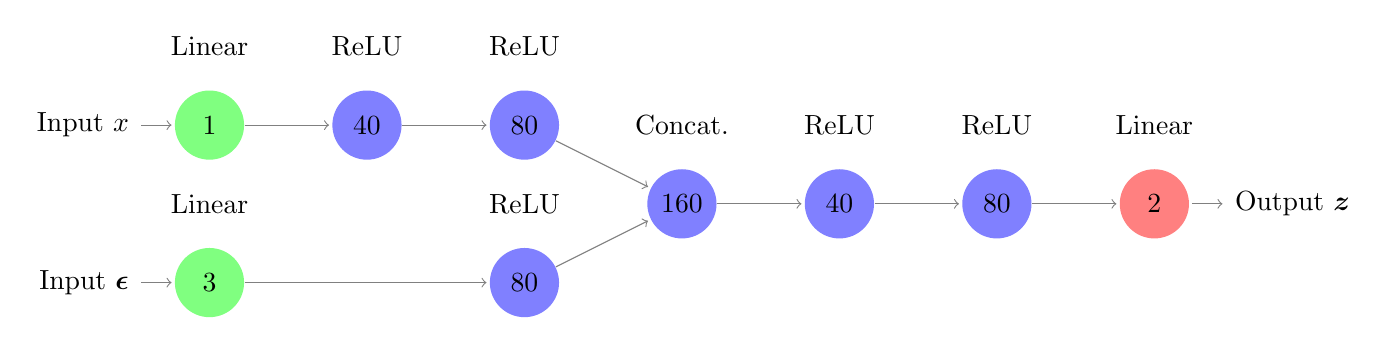
\begin{tikzpicture}[shorten >=1pt,->,draw=black!50, node distance=2.5cm]
    \tikzstyle{every pin edge}=[<-,shorten <=1pt]
    \tikzstyle{neuron}=[circle,fill=black!25,minimum size=25pt,inner sep=0pt]
    \tikzstyle{input neuron}=[neuron, fill=green!50];
    \tikzstyle{output neuron}=[neuron, fill=red!50];
    \tikzstyle{hidden neuron}=[neuron, fill=blue!50];
    \tikzstyle{annot} = [text width=4em, text centered]
    
	%\node[input neuron, pin=left:Bias] (I-0) at (0,0) {$x_0$};
    % Draw the input layer nodes
    %\foreach \name / \y in {1,...,3}
    % This is the same as writing \foreach \name / \y in {1/1,2/2,3/3,4/4}
    \node[input neuron, pin=left:Input $x$] (I-1) at (0,-1) {$1$};
	\node[input neuron, pin=left:Input $\bm{\epsilon}$] (I-2) at (0,-3) {$3$};

    \path[yshift=0cm] node[hidden neuron] (H-11) at (2.0cm,-1) {$40$};
	\path[yshift=0cm] node[hidden neuron] (H-12) at (4.0cm,-1) {$80$};
    \path[yshift=0cm] node[hidden neuron] (H-2) at (4.0cm,-3) {$80$};
    \path[yshift=0cm] node[hidden neuron] (H-3) at (6.0cm,-2) {$160$};
    \path[yshift=0cm] node[hidden neuron] (H-31) at (8.0cm,-2) {$40$};
    \path[yshift=0cm] node[hidden neuron] (H-32) at (10.0cm,-2) {$80$};
	\path[yshift=0cm] node[output neuron,pin={[pin edge={->}]right:Output $\bm{z}$}] (O) at (12.0cm, -2) {$2$};
    \path (I-1) edge (H-11);
    \path (H-11) edge (H-12);
	\path (I-2) edge (H-2);
	\path (H-12) edge (H-3);
	\path (H-2) edge (H-3);
	\path (H-3) edge (H-31);
	\path (H-31) edge (H-32);
	\path (H-32) edge (O);
    % Annotate the layers
    \node[annot,above of=I-1, node distance=1cm] {Linear};
    \node[annot,above of=I-2, node distance=1cm] {Linear};
    \node[annot,above of=H-11, node distance=1cm] {ReLU};
    \node[annot,above of=H-12, node distance=1cm] {ReLU};
    \node[annot,above of=H-2, node distance=1cm] {ReLU};
    \node[annot,above of=H-3, node distance=1cm] {Concat.};
    \node[annot,above of=H-31, node distance=1cm] {ReLU};
    \node[annot,above of=H-32, node distance=1cm] {ReLU};
    \node[annot,above of=O, node distance=1cm] {Linear};
\end{tikzpicture}\\
The number inside the node indicates how many nodes the layer has, and the text above the node describes the activation function in the layer. Recall that the input layer does not have an activation function (Linear), and Rectified Linear Units (ReLU) are used for most of the hidden layers due to their many advantages. In the Concat. layer, the two input vectors are concatenated and there is no activation function placed on the layer. Since arbitrary probability distribution samples can take any real number, we do not use an activation function for the output layer.\\
\\
The structure of the estimator (discriminator $\mathcal{D}_\alpha(z,x)$ or ratio estimator $\mathcal{R}_\alpha(z,x)$) is similar to that of the the generator, with an additional hidden layer associated with the $z$ input and a different activation function for the output layer, corresponding to the estimator's identity. Note that in terms of code, the only differences between class probability estimation and divergence minimisation are the activation function of the estimator's output layer and the loss functions being minimised. A sigmoid output layer is used for a discriminator, whilst a rectified linear output is used for a ratio estimator. The estimator structure is shown in Figure below:\\
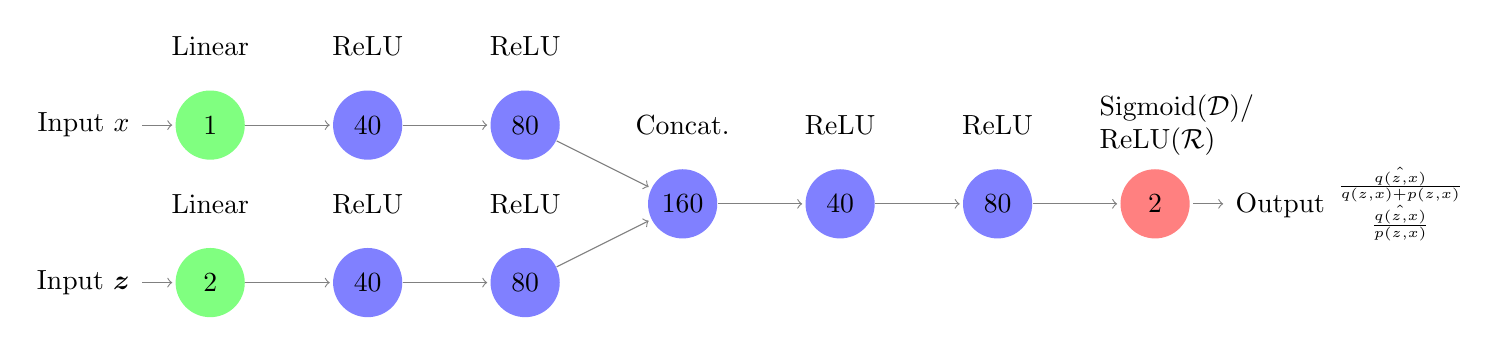
\begin{tikzpicture}[shorten >=1pt,->,draw=black!50, node distance=2.5cm]
    \tikzstyle{every pin edge}=[<-,shorten <=1pt]
    \tikzstyle{neuron}=[circle,fill=black!25,minimum size=25pt,inner sep=0pt]
    \tikzstyle{input neuron}=[neuron, fill=green!50];
    \tikzstyle{output neuron}=[neuron, fill=red!50];
    \tikzstyle{hidden neuron}=[neuron, fill=blue!50];
    \tikzstyle{annot} = [text width=4em, text centered]
    
	%\node[input neuron, pin=left:Bias] (I-0) at (0,0) {$x_0$};
    % Draw the input layer nodes
    %\foreach \name / \y in {1,...,3}
    % This is the same as writing \foreach \name / \y in {1/1,2/2,3/3,4/4}
    \node[input neuron, pin=left:Input $x$] (I-1) at (0,-1) {$1$};
	\node[input neuron, pin=left:Input $\bm{z}$] (I-2) at (0,-3) {$2$};

    \path[yshift=0cm] node[hidden neuron] (H-11) at (2.0cm,-1) {$40$};
	\path[yshift=0cm] node[hidden neuron] (H-12) at (4.0cm,-1) {$80$};
	\path[yshift=0cm] node[hidden neuron] (H-21) at (2.0cm,-3) {$40$};
    \path[yshift=0cm] node[hidden neuron] (H-22) at (4.0cm,-3) {$80$};
    \path[yshift=0cm] node[hidden neuron] (H-3) at (6.0cm,-2) {$160$};
    \path[yshift=0cm] node[hidden neuron] (H-31) at (8.0cm,-2) {$40$};
    \path[yshift=0cm] node[hidden neuron] (H-32) at (10.0cm,-2) {$80$};
	\path[yshift=0cm] node[output neuron,pin={[pin edge={->}]right:Output $\genfrac{}{}{0pt}{}{\hat{\frac{q(z,x)}{q(z,x)+p(z,x)}}}{\hat{\frac{q(z,x)}{p(z,x)}}}$}] (O) at (12.0cm, -2) {$2$};
    \path (I-1) edge (H-11);
    \path (H-11) edge (H-12);
	\path (I-2) edge (H-21);
	\path (H-21) edge (H-22);
	\path (H-12) edge (H-3);
	\path (H-22) edge (H-3);
	\path (H-3) edge (H-31);
	\path (H-31) edge (H-32);
	\path (H-32) edge (O);
    % Annotate the layers
    \node[annot,above of=I-1, node distance=1cm] {Linear};
    \node[annot,above of=I-2, node distance=1cm] {Linear};
    \node[annot,above of=H-11, node distance=1cm] {ReLU};
    \node[annot,above of=H-12, node distance=1cm] {ReLU};
    \node[annot,above of=H-21, node distance=1cm] {ReLU};
    \node[annot,above of=H-22, node distance=1cm] {ReLU};
    \node[annot,above of=H-3, node distance=1cm] {Concat.};
    \node[annot,above of=H-31, node distance=1cm] {ReLU};
    \node[annot,above of=H-32, node distance=1cm] {ReLU};
    \node[annot,above of=O, node distance=1cm] {Sigmoid($\mathcal{D}$)/ ReLU($\mathcal{R}$)};
\end{tikzpicture}\\
The network weights are initialized with Xavier initialization, and trained using the Adam optimizer with learning rate $0.00001$. This is the highest learning rate at which both algorithms converge consistently; any higher learning rates lead to inconsistent results. The network is only trained on the data values $x=0,5,8,12,50$; in each training iteration, 400 samples are taken for each x-value, corresponding to a batch size of 2000. This relatively large batch size makes training more consistent, as performing back-propagation along a stochastic neural network can lead to random and erratic training. To prevent problems associated with taking $\log 0$, we add a small constant $c=10^{-18}$ to the log function's input. The estimator is pre-trained for 5000 iterations to ensure that it converges to its optimal value. This is particularly desired as training the generator with an inaccurate ELBO estimate is pointless. Afterwards, the program runs for 50000 iterations, alternating between 80 training steps of the estimator and 1 training step of the generator. This process for class probability estimation and divergence minimisation is shown in Algorithm and Algorithm below:
\begin{algorithm}
\SetKw{update}{update}
\caption{Sprinkler Prior-Contrastive Class Probability Estimation}
\KwData{Dataset $q^*(x)=\{0,5,8,12,20\}$, true (implicit) prior $p(z)\sim \mathcal{N}(0,2I_{2\times 2})$, true (implicit) likelihood $p(x|z)\sim EXP(3+\max(0,z_1)^3+\max(0,z_2)^3)$, noise distribution $\pi(\epsilon)\sim \mathcal{N}(0,I_{3\times 3})$}
\KwResult{Optimized posterior generator $\mathcal{G}_\phi(\epsilon;x)$}
\BlankLine
\For{$j=1$ \KwTo $5001$}{
	Sample $\{\epsilon^{(i,j)}\}^{2000}_{i=1}\sim \pi(\epsilon)$\;
		Sample $\{0,5,8,12,50\}^{400}_{i=1}=\{x^{(i,j)}\}^{2000}_{i=1}\sim q^*(x)$\;
		Sample $\{z^{(i,j)}_p\}^{2000}_{i=1}\sim p(z)$\;
		\ForEach{$\epsilon^{(i,j)},x^{(i,j)}$}{
			Sample $\{z^{(i,j)}_q\}^{2000}_{i=1}=\mathcal{G}(\epsilon^{(i,j)};x^{(i,j}_q)$\;
		}
		\update{$\alpha$ by optimization step on}{
			$\min_\alpha -\frac{1}{2000}\sum_{i=1}^{2000}\{\log [D_\alpha(\mathcal{G}_\phi(\epsilon^{(i,j)};x^{(i,j)}), x^{(i,j)})]+\log [1-D_\alpha(z_p^{(i,j)},x^{(i,j)})]\}$\;
		}
}
\For{$j=1$ \KwTo $50001$}{
	\For{$k=1$ \KwTo $80$}{	
		Sample $\{\epsilon^{(i,k)}\}^{2000}_{i=1}\sim \pi(\epsilon)$\;
		Sample $\{0,5,8,12,50\}^{400}_{i=1}=\{x^{(i,k)}\}^{2000}_{i=1}\sim q^*(x)$\;
		Sample $\{z^{(i,k)}_p\}^{2000}_{i=1}\sim p(z)$\;
		\ForEach{$\epsilon^{(i,k)},x^{(i,k)}$}{
			Sample $\{z^{(i,k)}_q\}^{2000}_{i=1}=\mathcal{G}(\epsilon^{(i,k)};x^{(i,k)}_q)$\;
		}
		\update{$\alpha$ by optimization step on}{
			$\min_\alpha -\frac{1}{2000}\sum_{i=1}^{2000}\{\log [D_\alpha(\mathcal{G}_\phi(\epsilon^{(i,k)};x^{(i,k)}), x^{(i,k)})]+\log [1-D_\alpha(z_p^{(i,k)},x^{(i,k)})]\}$\;
		}
	}
	Sample $\{\epsilon^{(i)}\}^{2000}_{i=1}\sim \pi(\epsilon)$\;
	Sample $\{0,5,8,12,50\}^{400}_{i=1}=\{x^{(i)}\}^{2000}_{i=1}\sim q^*(x)$\;
	\update{$\phi$ by optimization step on}{
		$\min_\phi \frac{1}{2000}\sum^{2000}_{i=1}\{-\log p(x|\mathcal{G}_\phi(\epsilon^{(i)};x^{(i)}))+\log\frac{D_\alpha(\mathcal{G}_\phi(\epsilon^{(i)};x^{(i)}),x^{(i)})}{1-D_\alpha(\mathcal{G}_\phi(\epsilon^{(i)};x^{(i)}),x^{(i)})}\}$\;
	}
}
\end{algorithm}
\begin{algorithm}
\SetKw{update}{update}
\caption{Sprinkler Prior-Contrastive KL Divergence Minimisation}
\KwData{Dataset $q^*(x)=\{0,5,8,12,20\}$, true (implicit) prior $p(z)\sim \mathcal{N}(0,2I_{2\times 2})$, true (implicit) likelihood $p(x|z)\sim EXP(3+\max(0,z_1)^3+\max(0,z_2)^3)$, noise distribution $\pi(\epsilon)\sim \mathcal{N}(0,I_{3\times 3})$}
\KwResult{Optimized posterior generator $\mathcal{G}_\phi(\epsilon;x)$}
\BlankLine
\For{$j=1$ \KwTo $5001$}{
	Sample $\{\epsilon^{(i,j)}\}^{2000}_{i=1}\sim \pi(\epsilon)$\;
		Sample $\{0,5,8,12,50\}^{400}_{i=1}=\{x^{(i,j)}\}^{2000}_{i=1}\sim q^*(x)$\;
		Sample $\{z^{(i,j)}_p\}^{2000}_{i=1}\sim p(z)$\;
		\ForEach{$\epsilon^{(i,j)},x^{(i,j)}$}{
			Sample $\{z^{(i,j)}_q\}^{2000}_{i=1}=\mathcal{G}(\epsilon^{(i,j)};x^{(i,j})$\;
		}
		\update{$\alpha$ by optimization step on}{
			$\min_\alpha -\frac{1}{2000}\sum_{i=1}^{2000}\{\log [r_\alpha(\mathcal{G}_\phi(\epsilon^{(i,j)};x^{(i,j)}), x^{(i,j)})]+r_\alpha(z_p^{(i,j)},x^{(i,j)})\}$\;
		}
}
\For{$j=1$ \KwTo $50001$}{
	\For{$k=1$ \KwTo $80$}{	
		Sample $\{\epsilon^{(i,k)}\}^{2000}_{i=1}\sim \pi(\epsilon)$\;
		Sample $\{0,5,8,12,50\}^{400}_{i=1}=\{x^{(i,k)}\}^{2000}_{i=1}\sim q^*(x)$\;
		Sample $\{z^{(i,k)}_p\}^{2000}_{i=1}\sim p(z)$\;
		\ForEach{$\epsilon^{(i,k)},x^{(i,k)}$}{
			Sample $\{z^{(i,k)}_q\}^{2000}_{i=1}=\mathcal{G}(\epsilon^{(i,k)};x^{(i,k)}_q)$\;
		}
		\update{$\alpha$ by optimization step on}{
			$\min_\alpha -\frac{1}{2000}\sum_{i=1}^{2000}\{\log [r_\alpha(\mathcal{G}_\phi(\epsilon^{(i,k)};x^{(i,k)}), x^{(i,k)})]+r_\alpha(z_p^{(i,k)},x^{(i,k)})\}$\;
		}
	}
	Sample $\{\epsilon^{(i)}\}^{2000}_{i=1}\sim \pi(\epsilon)$\;
	Sample $\{0,5,8,12,50\}^{400}_{i=1}=\{x^{(i)}\}^{2000}_{i=1}\sim q^*(x)$\;
	\update{$\phi$ by optimization step on}{
		$\min_\phi \frac{1}{2000}\sum^{2000}_{i=1}\{-\log p(x|\mathcal{G}_\phi(\epsilon^{(i)};x^{(i)}))+\log r_\alpha(\mathcal{G}_\phi(\epsilon^{(i)};x^{(i)}),x^{(i)})\}$\;
	}
}
\end{algorithm}
\begin{algorithm}
\SetKw{update}{update}
\caption{Sprinkler Joint-Contrastive Class Probability Estimation}
\KwData{Dataset $q^*(x)=\{0,5,8,12,20\}$, true (implicit) prior $p(z)\sim \mathcal{N}(0,2I_{2\times 2})$, true (implicit) likelihood $p(x|z)\sim EXP(3+\max(0,z_1)^3+\max(0,z_2)^3)$, noise distribution $\pi(\epsilon)\sim \mathcal{N}(0,I_{3\times 3})$}
\KwResult{Optimized posterior generator $\mathcal{G}_\phi(\epsilon;x)$}
\BlankLine
\For{$j=1$ \KwTo $5001$}{
	Sample $\{\epsilon^{(i,j)}\}^{2000}_{i=1}\sim \pi(\epsilon)$\;
		Sample $\{0,5,8,12,50\}^{400}_{i=1}=\{x^{(i,j)}_q\}^{2000}_{i=1}\sim q^*(x)$\;
		Sample $\{z^{(i,j)}_p\}^{2000}_{i=1}\sim p(z)$\;
		\ForEach{$\epsilon^{(i,j)},x^{(i,j)}$}{
			Sample $\{z^{(i,j)}_q\}^{2000}_{i=1}=\mathcal{G}(\epsilon^{(i,j)};x^{(i,j}_q)$\;
		}
		\ForEach{$z^{(i,j)}_p$}{
			Sample $\{x^{(i,j)}_p\}^{2000}_{i=1}\sim p(x|z)$\;
		}
		\update{$\alpha$ by optimization step on}{
			$\min_\alpha -\frac{1}{2000}\sum_{i=1}^{2000}\{\log [D_\alpha(\mathcal{G}_\phi(\epsilon^{(i,j)};x_q^{(i,j)}), x_q^{(i,j)})]+\log [1-D_\alpha(z_p^{(i,j)},x_p^{(i,j)})]\}$\;
		}
}
\For{$j=1$ \KwTo $50001$}{
	\For{$k=1$ \KwTo $80$}{	
		Sample $\{\epsilon^{(i,k)}\}^{2000}_{i=1}\sim \pi(\epsilon)$\;
		Sample $\{0,5,8,12,50\}^{400}_{i=1}=\{x^{(i,k)}_q\}^{2000}_{i=1}\sim q^*(x)$\;
		Sample $\{z^{(i,k)}_p\}^{2000}_{i=1}\sim p(z)$\;
		\ForEach{$\epsilon^{(i,k)},x^{(i,k)}$}{
			Sample $\{z^{(i,k)}_q\}^{2000}_{i=1}=\mathcal{G}(\epsilon^{(i,k)};x^{(i,k)}_q)$\;
		}
		\ForEach{$z^{(i,k)}_p$}{
			Sample $\{x^{(i,k)}_p\}^{2000}_{i=1}\sim p(x|z)$\;
		}
		\update{$\alpha$ by optimization step on}{
			$\min_\alpha -\frac{1}{2000}\sum_{i=1}^{2000}\{\log [D_\alpha(\mathcal{G}_\phi(\epsilon^{(i,k)};x_q^{(i,k)}), x_q^{(i,k)})]+\log [1-D_\alpha(z_p^{(i,k)},x_p^{(i,k)})]\}$\;
		}
	}
	Sample $\{\epsilon^{(i)}\}^{2000}_{i=1}\sim \pi(\epsilon)$\;
	Sample $\{0,5,8,12,50\}^{400}_{i=1}=\{x^{(i)}_q\}^{2000}_{i=1}\sim q^*(x)$\;
	\update{$\phi$ by optimization step on}{
		$\min_\phi \frac{1}{2000}\sum^{2000}_{i=1}\log\frac{D_\alpha(\mathcal{G}_\phi(\epsilon^{(i)};x_q^{(i)}),x_q^{(i)})}{1-D_\alpha(\mathcal{G}_\phi(\epsilon^{(i)};x_q^{(i)}),x_q^{(i)})}$\;
	}
}
\end{algorithm}
\begin{algorithm}
\SetKw{update}{update}
\caption{Sprinkler Joint-Contrastive KL Divergence Minimisation}
\KwData{Dataset $q^*(x)=\{0,5,8,12,20\}$, true (implicit) prior $p(z)\sim \mathcal{N}(0,2I_{2\times 2})$, true (implicit) likelihood $p(x|z)\sim EXP(3+\max(0,z_1)^3+\max(0,z_2)^3)$, noise distribution $\pi(\epsilon)\sim \mathcal{N}(0,I_{3\times 3})$}
\KwResult{Optimized posterior generator $\mathcal{G}_\phi(\epsilon;x)$}
\BlankLine
\For{$j=1$ \KwTo $5001$}{
	Sample $\{\epsilon^{(i,j)}\}^{2000}_{i=1}\sim \pi(\epsilon)$\;
		Sample $\{0,5,8,12,50\}^{400}_{i=1}=\{x^{(i,j)}_q\}^{2000}_{i=1}\sim q^*(x)$\;
		Sample $\{z^{(i,j)}_p\}^{2000}_{i=1}\sim p(z)$\;
		\ForEach{$\epsilon^{(i,j)},x^{(i,j)}$}{
			Sample $\{z^{(i,j)}_q\}^{2000}_{i=1}=\mathcal{G}(\epsilon^{(i,j)};x^{(i,j}_q)$\;
		}
		\ForEach{$z^{(i,j)}_p$}{
			Sample $\{x^{(i,j)}_p\}^{2000}_{i=1}\sim p(x|z)$\;
		}
		\update{$\alpha$ by optimization step on}{
			$\min_\alpha -\frac{1}{2000}\sum_{i=1}^{2000}\{\log [r_\alpha(\mathcal{G}_\phi(\epsilon^{(i,j)};x_q^{(i,j)}), x_q^{(i,j)})]+r_\alpha(z_p^{(i,j)},x_p^{(i,j)})\}$\;
		}
}
\For{$j=1$ \KwTo $50001$}{
	\For{$k=1$ \KwTo $80$}{	
		Sample $\{\epsilon^{(i,k)}\}^{2000}_{i=1}\sim \pi(\epsilon)$\;
		Sample $\{0,5,8,12,50\}^{400}_{i=1}=\{x^{(i,k)}_q\}^{2000}_{i=1}\sim q^*(x)$\;
		Sample $\{z^{(i,k)}_p\}^{2000}_{i=1}\sim p(z)$\;
		\ForEach{$\epsilon^{(i,k)},x^{(i,k)}$}{
			Sample $\{z^{(i,k)}_q\}^{2000}_{i=1}=\mathcal{G}(\epsilon^{(i,k)};x^{(i,k)}_q)$\;
		}
		\ForEach{$z^{(i,k)}_p$}{
			Sample $\{x^{(i,k)}_p\}^{2000}_{i=1}\sim p(x|z)$\;
		}
		\update{$\alpha$ by optimization step on}{
			$\min_\alpha -\frac{1}{2000}\sum_{i=1}^{2000}\{\log [r_\alpha(\mathcal{G}_\phi(\epsilon^{(i,k)};x_q^{(i,k)}), x_q^{(i,k)})]+r_\alpha(z_p^{(i,k)},x_p^{(i,k)})\}$\;
		}
	}
	Sample $\{\epsilon^{(i)}\}^{2000}_{i=1}\sim \pi(\epsilon)$\;
	Sample $\{0,5,8,12,50\}^{400}_{i=1}=\{x^{(i)}_q\}^{2000}_{i=1}\sim q^*(x)$\;
	\update{$\phi$ by optimization step on}{
		$\min_\phi \frac{1}{2000}\sum^{2000}_{i=1}\log r_\alpha(\mathcal{G}_\phi(\epsilon^{(i)};x_q^{(i)}),x_q^{(i)})$\;
	}
}
\end{algorithm}
\newpage
\subsubsection{Results}
To compare the techniques, we compare the number of iterations until convergence and how much the variational posterior has converged after x0000 iterations. We define convergence as when the average KL divergence of the 5 posterior distributions $\E_{q^*(x)}KL(q(z|x)||p(z|x)) = \E_{q^*(x)}\E_{q(z|x)}\log \frac{q(z|x)}{p(z|x)}$ falls below 1.35. We do not use the ELBO output of the program to calculate this KL divergence, nor do we compare the ELBOs of the algorithms, as the accuracy of the ELBO estimator is dependent on the algorithm used. Instead, we use a non-parametric approach, estimating the probability density function of the variational posterior output with a Gaussian kernel density estimator $\hat{q}(z|x)$. By using five kernel density estimators for the five data points, we are able to create an estimate of the average KL divergence with an accuracy that is independent of the algorithm used: $\E_{q^*(x)}KL(\hat{q}(z|x)||p(z|x)) = \E_{q^*(x)}\E_{q(z|x)}\log \frac{\hat{q}(z|x)}{p(z|x)}$.\\
Clearly, the prior-contrastive algorithms converged much faster their joint-contrastive equivalent, as expected since knowledge of the likelihood improves posterior optimization. Overall, for both PC and JC, we found that class probability estimation performed consistently better than KL divergence minimisation. Insert metrics here. Each iteration took approximately the same amount of time to compute (0.32 seconds on me PC), as the bulk of the training time is spent training the neural networks, which have similar structures.\\
Furthermore, in approximately half of the simulations, the ratio loss of the KL divergence minimisation algorithm would start at a relatively high number (42.3 as opposed to 3.5), and it would be stuck there for the entire runtime of the program; the thousands of iterations spent minimizing the ratio loss had little effect decreasing it (the pre-training period of 5000 iterations only lowered the ratio loss to about 39.2). The high ratio loss signifies a very inaccurate ratio estimator, leading to a completely inaccurate variational posterior (i have a fig to isnert here). Thus, the program would have to be restarted every time the ratio loss initialized at a high number, until a reasonable value was initialized. 
\newpage
\subsection{Theorycraftintime}
In an attempt to explain why class probability estimation is significantly superior to KL minimization, we compare the two techniques in terms of their 'lower bound' formulation, and analyze their fundamental differences.
\subsubsection{Introduction to my mad theory}
For both the prior-contrastive and joint-contrastive formulations, it can be seen that the only differences between CPE and KL min are the function that is optimized to formulate the density ratio estimator, and the parametrization of the estimator. Recall that optimization of the estimator for the KL min algorithm follows the lower bound:
\[D_{KL}(p||q)\geq \sup_{\alpha}\{\mathbb{E}_{q(u)}[1+\log r_\alpha(u)]-\mathbb{E}_{p(u)}[r_\alpha(u)]\}\]
with equality at $r_\alpha(u)=\frac{q(u)}{p(u)}$ and that optimization for class probability estimation follows:
\[2D_{JS}(p||q)-\log 4\geq \sup_\alpha\{\mathbb{E}_{q(u)}[\log \mathcal{D}_\alpha(u)]+\mathbb{E}_{p(u)}[\log(1-\mathcal{D}_\alpha(u))]\}\]
with equality at $D_\alpha(u)=\frac{q(u)}{q(u)+p(u)}$.\\
These two estimators can be used interchangeably, as $D_\alpha(u)=\frac{r_\alpha(u)}{r_\alpha(u)+1}$ and $r_\alpha(u)=\frac{D_\alpha(u)}{1-D_\alpha(u)}$. In fact, the former transformation is used to derive this formulation of the discriminative loss for class probability estimation. By transforming the estimators used in the two f-divergences, we can formulate two new estimator optimization problems:
\[\min_\alpha \mathbb{E}_{q(u)}[\log D_\alpha (u)-\log(1-D_\alpha(u))]-\mathbb{E}_{p(u)}\frac{D_\alpha(u)}{1-D_\alpha(u)}\]
and
\[\min_\alpha -\mathbb{E}_{q(u)}[\log r_\alpha(u)-\log (r_\alpha(u)+1)]+\mathbb{E}_{p(u)}[\log(r_\alpha(u)+1)].\]
The optimization problem for the ELBO in both prior-contrastive and joint-contrastive methods involves density ratio estimation between the true and variational distributions, and the optimization of the likelihood term in the prior-contrastive method is independent of the ratio estimator. We can therefore denote the two ELBO optimization problems for the two estimator parametrizations $D_\alpha (u)$ and $r_\alpha(u)$ as:
\[\min_\phi \mathbb{E}_{q_\phi(u)}\log \frac{D_\alpha (u)}{1-D_\alpha (u)}\quad(+\text{ Likelihood})\]
and
\[\min_\phi \mathbb{E}_{q_\phi(u)}\log r_\alpha (u)\quad(+\text{ Likelihood}).\]
Additionally, we can parametrize the estimator such that it estimates the log ratio directly: $T_\alpha(u)=\log r_\alpha(u)$. This simplifies the objective function for our variational neural network weights to:
\[\min_\phi -\mathbb{E}_{q_\phi(u)}[T_\alpha(u)]\quad(+\text{ Likelihood}).\]
For the KL Divergence, the estimator is optimized as follows:
\[\min_\alpha -\mathbb{E}_{q(u)}[T_\alpha(u)]+\mathbb{E}_{p(u)}[e^{T_\alpha (u)}]\]
The CPE divergence equivalent is:
\[\min_\alpha -\E_{q(u)}\left[\log \frac{e^{T_\alpha(u)}}{e^{T_\alpha(u)}+1}\right]+\E_{p(u)}[\log(e^{T_\alpha(u)}+1)]\]
\subsubsection{Recap because its confusing}
To recap, we have mathematically simplified the choice of algorithm for training ratio estimators for implicit variational neural networks to a choice of f-divergence:
\begin{itemize}
\item KL Divergence: $D_{KL}(p||q)=\mathbb{E}_{q(u)}[1+\log \frac{q(u)}{p(u)}]-\mathbb{E}_{p(u)}\left[\frac{q(u)}{p(u)}\right]$
\item CPE Divergence: $D_{CPE}(p||q)=\mathbb{E}_{q(u)}\left[\log \frac{q(u)}{q(u)+p(u)}\right]+\mathbb{E}_{p(u)}\left[\log \frac{p(u)}{q(u)+p(u)}\right]$
\end{itemize}
and a choice of estimator parametrization:
\begin{itemize}
\item Direct ratio estimator: $r^*_\alpha(u)=\frac{q(u)}{p(u)}$
\item "Class probability" estimator: $D^*_\alpha(u)=\frac{q(u)}{q(u)+p(u)}$
\item Direct log ratio estimator: $T^*_\alpha(u)=\log \frac{q(u)}{p(u)}$
\end{itemize}
The original "KL minimization approach" simply chooses the KL Divergence and the direct ratio estimator, and "Class probability estimation" uses the CPE Divergence and the "Class probability" estimator. These are just 2 variations of the 6 available algorithms.
\subsubsection{First and Second Derivatives of all 6 possible algorithms}
To evaluate the effectiveness of gradient descent optimization in these algorithms, we formulate the first and second derivatives of the objective functions. We first take the "Class probability" parametrization and observe its optimization problem for the CPE divergence:
\begin{align*}
f_{CPE}(u)&=-\E_{q(u)}[\log D(u)]-\E_{p(u)}[\log (1-D(u))]\\
&=-\int_u q(u)\log D(u) du -\int_u p(u)\log(1-D)du\\
\frac{df}{dD(u)}&=-\frac{q(u)}{D(u)}+\frac{p(u)}{1-D(u)}\\
\frac{d^2f}{dD^2(u)}&=\frac{q(u)}{D^2(u)}+\frac{p(u)}{(1-D(u))^2}\\
&>0 \quad \forall q(u)\in(0,1), p(u)\in (0,1), D(u)\in (0,1) 
\end{align*}
Since the second derivative is always greater than zero, the function is strictly convex and therefore converges linearly with gradient descent.\\
Now observe the optimization problem for the KL Divergence:
\begin{align*}
f_{KL}(u)&=-\E_{q(u)}\left(\log \frac{D(u)}{1-D(u)}\right)+\E_{p(u)}\left(\frac{D(u)}{1-D(u)}\right)\\
&=-\int_u q(u)\left(\log \frac{D(u)}{1-D(u)}\right)du+\int_u p(u)\left(\frac{D(u)}{1-D(u)}\right)du\\
\frac{df}{dD(u)}&=-\frac{q(u)}{D(u)}-\frac{q(u)}{1-D(u)}+\frac{p(u)}{1-D(u)}+\frac{p(u)D(u)}{(1-D(u))^2}\\
&=-\frac{q(u)}{D(u)}-\frac{q(u)}{1-D(u)}+\frac{p(u)}{(1-D(u))^2}\\
\frac{d^2f}{dD^2(u)}&=\frac{q(u)}{D^2(u)}-\frac{q(u)}{(1-D(u))^2}+\frac{2p(u)}{(1-D(u))^3}
\end{align*}
CPE with ratio parametrisation:
\begin{align*}
f_{CPE}(u)&=-\E_{q(u)}\left[\log \frac{r(u)}{r(u)+1}\right]+\E_{p(u)}\left[\log(r(u)+1)\right]\\
&=-\int_u q(u)\left[\log \frac{r(u)}{r(u)+1}\right]du+\int_u p(u)\left[\log(r(u)+1)\right]du\\
\frac{df}{dr(u)}&=-\frac{q(u)}{r(u)}+\frac{q(u)}{r(u)+1}+\frac{p(u)}{r(u)+1}\\
\frac{d^2f}{dr^2(u)}&=\frac{q(u)}{r^2(u)}-\frac{q(u)}{(r(u)+1)^2}-\frac{p(u)}{(r(u)+1)^2}
\end{align*}
KL with ratio parametrisation:
\begin{align*}
f_{KL}(u)&=-\E_{q(u)}(\log r(u))+\E_{p(u)}r\\
&=-\int_u q(u)\log r(u) du+\int_u p(u)r(u)du\\
\frac{df}{dr(u)}&=-\frac{q(u)}{r(u)}+p(u)\\
\frac{d^2f}{dr^2(u)}&=\frac{q(u)}{r^2(u)}\\
&>0
\end{align*}
CPE with log ratio parametrisation:
\begin{align*}
f_{CPE}(u)&=-\E_{q(u)}[T(u)-\log(e^{T(u)}+1)]+\E_{p(u)}[\log(e^{T(u)}+1)]\\
&=\int_u q(u)[\log(e^{T(u)}+1)-T(u)] du+\int_u p(u)[\log(e^{T(u)}+1)]du\\
\frac{df}{dT(u)}&=-q(u)+\frac{(q(u)+p(u))e^{T(u)}}{e^{T(u)}+1}\\
\frac{d^2f}{dT^2(u)}&=\frac{(q(u)+p(u))\exp(T(u))}{e^{T(u)}+1}-\frac{(q(u)+p(u))e^{2T(u)}}{(e^{T(u)}+1)^2}\\
&=\frac{(q(u)+p(u))(e^{2T(u)}+e^{T(u)})-(q(u)+p(u))e^{2T(u)}}{(e^{T(u)}+1)^2}\\
&=\frac{(q(u)+p(u))e^{T(u)}}{(e^{T(u)}+1)^2}\\
&>0
\end{align*}
KL with log ratio parametrisation:
\begin{align*}
f_{KL}(u)&=-\E_{q(u)}[T(u)]+\E_{p(u)}[e^{T(u)}]\\
&=-\int_u q(u)T(u)du+\int_u p(u)e^{T(u)}du\\
\frac{df}{dT(u)}&=-q(u)+p(u)e^{T(u)}\\
\frac{d^2f}{dT^2(u)}&=p(u)e^{T(u)}\\
&>0
\end{align*}
\subsubsection{Difference between divergences}
Recall that both divergences attain the same global minimum, which is a parametrization of the estimator, and that these estimators are optimized via stochastic gradient descent. Thus, for a fixed estimator parametrization, the divergences will have varying rates of convergence, which can be analyzed by observing the second derivative. The convergence rate of a gradient descent method is proportional to the size of its second derivative. Due to the variable nature of $p(u)$, $q(u)$ and $D(u)$/$r(u)$/$T(u)$, it is uncertain whether a divergence is superior in this aspect when its second derivative is not strictly greater than the other divergence's equivalent. We are therefore unable to arrive at a certain conclusion for the "Class probability" and direct log ratio estimators, but it can be seen that in the direct ratio parametrisation, the KL divergence is strictly greater than the CPE divergence, implying that it would be superior. However, due to the significant number of iterations taken for each estimator optimization step, it is unlikely the different divergences have a significant impact on the quality of the method. This can be additionally seen in the non-significant decrease in estimator loss over the later half of its optimization step.
\subsubsection{Difference between estimators}
Again, we compare the second derivatives of the techniques, this time fixing the divergence and observing the difference in estimator parametrization. Due to the exponential term in the log ratio parametrisation, no conclusion can be drawn from its comparisons. We cannot conclude anything from comparing the remaining two estimators for the KL divergence either. It can however be seen that for the CPE divergence, the "Class probability" parametrization is strictly superior.\\
Now consider the bounds on the 

We now address the "failures" experienced by the KL minimization algorithm. Consider that the activation function of the estimator network's output layer, influencing the output range, varies between the estimators. For the direct ratio estimator, ReLU is used for the output, meaning that a 0 is outputted if the previous matrix operations lead to a negative number. Now recall that we take the log of the ratio estimator's output in all of the related optimization problems, and that a small constant $c$ is added to prevent taking the log of $0$. This explains the 'failures' of the KL minimization algorithm: the neural network has been initialised such that a $0$ is outputted, signifying that the previous matrix operations led to a negative number. Its loss function takes a large value according to this scenario (e.g. for KL minimization, it is $-\log c$), and does not decrease over training iterations, as a slight change in the network weights would still output the same result, meaning that the partial derivative of the weights with respect to the loss function is $0$. Due to this occurrence, the "failures" would additionally occur in the direct log ratio estimator, as its output layer is simply the log of a ReLU output, which would suffer from the same problem. On the other hand, the sigmoid activation function of the "Class probability" estimator is bound in $(0,1)$, so it does not experience any "failures".\\
Aside from the failures, the difference in output activation functions could also explain our experimental results; the rectified linear unit models the density ratio in a linear manner, meaning that it would be asymmetric, in the sense that cases where $q(u)>p(u)$ result in any output in $(1,\infty)$, but if $p(u)<q(u)$, then the outputted is limited to $(0,1)$. On the other hand, the sigmoid function has symmetric output, as if $q(u)>p(u)$, it is bound in $(0.5,1)$, and if $q(u)<p(u)$, the outputs lie within $(0,0.5)$. Taking the log of the rectified linear output and optimizing the objective functions with respect to it may partially resolve this issue, as the cases will become bound in $(0,\infty)$ and $(-\infty,0)$ respectively, but it would retain an additional issue: having a rectified linear unit for the output layer restricts the previous matrix operations to have an output in $\R^{+}\backslash \{0\}$, as its surjective mapping truncates $\R^-$. On the other hand, the sigmoid output layer has a bijective mapping from $\R$ to $(0,1)$.
\subsection{Experiments to prove me theory}
\subsection{Adversarial Variational Bayes (MNIST image generation)}
\subsubsection{Problem Context}
\section{Related Work and Discussion}
\section{Conclusion}
\end{document}
